%%% PLANTILLA DISEÑADA PARA LA REALIZACIÓN DE TESIS DE PRE-GRADO DE LA FIEECS
%% AUTOR DE LA PLANTILLA: Oswaldo Espinoza-Hurtado

\documentclass[12pt,a4paper,oneside]{report}

\usepackage[T1]{fontenc}
\usepackage{times}
\usepackage[utf8]{inputenc}
\usepackage{amsmath}
\usepackage{graphicx}
\usepackage[colorlinks=false]{hyperref}
\usepackage{multicol}
\usepackage{longtable}
\usepackage[refpages]{gloss}
\usepackage{float}
\usepackage{anysize}
\usepackage{appendix}
\usepackage{lscape}
\usepackage{pdflscape}
\usepackage{multirow}
\usepackage{listings}
\usepackage{color}
\usepackage{setspace}
\usepackage{enumerate} 

\usepackage[spanish]{babel}
\usepackage{apacite} 

\usepackage{graphicx}
\usepackage[svgnames]{xcolor}
\usepackage{booktabs}
\usepackage{lscape}
\usepackage{multirow}
\usepackage{afterpage}
\pagestyle{plain}
\usepackage{anysize}
\usepackage{here}

\usepackage{url}
\usepackage{amsmath}
\usepackage{mathtools}
\usepackage{mathrsfs}

\usepackage[spanish,onelanguage,ruled,vlined,linesnumbered,noresetcount]{algorithm2e}

\makeatletter
\newcommand{\AlgoResetCount}{\renewcommand{\@ResetCounterIfNeeded}{\setcounter{AlgoLine}{0}}}
\newcommand{\AlgoNoResetCount}{\renewcommand{\@ResetCounterIfNeeded}{}}
\newcounter{AlgoSavedLineCount}
\newcommand{\AlgoSaveLineCount}{\setcounter{AlgoSavedLineCount}{\value{AlgoLine}}}
\newcommand{\AlgoRestoreLineCount}{\setcounter{AlgoLine}{\value{AlgoSavedLineCount}}}
\makeatother

\usepackage{enumitem}

\usepackage{bigints}
\newcommand\dummy{\frac{a}{c}\,\mathrm{d}P}

\usepackage{subcaption}


\begin{document}

%----------------------------------------------------------------------------------------
%	CONFIGURACION
%----------------------------------------------------------------------------------------



\marginsize{2.5cm}{2.5cm}{3.0cm}{2.5cm}
\renewcommand*{\contentsname}{ÍNDICE}
\renewcommand*{\listtablename}{Índice de tablas}
\renewcommand*{\listfigurename}{Índice de figuras}
\renewcommand{\baselinestretch}{1.0}
\renewcommand{\appendixname}{Anexo}
\renewcommand{\appendixtocname}{Anexos}
\renewcommand{\appendixpagename}{Anexos}
\renewcommand{\thetable}{\arabic{chapter}.\arabic{table}}
\renewcommand*{\tablename}{Tabla}
\renewcommand*{\chaptername}{Capítulo}
\renewcommand*{\thechapter}{\Roman{chapter}}
\renewcommand{\thesection}{\arabic{chapter}.\arabic{section}}
\renewcommand{\figurename}{Figura}
\renewcommand{\thefigure}{\arabic{chapter}.\arabic{figure}}
\renewcommand{\theequation}{\arabic{chapter}.\arabic{equation}}


%----------------------------------------------------------------------------------------
%	PORTADA
%----------------------------------------------------------------------------------------

\begin{titlepage}
 
\begin{center}
 
 {\Large \bf UNIVERSIDAD NACIONAL DE INGENIERÍA}\\[0.5cm]
 
{\bf FACULTAD DE INGENIERÍA ECONÓMICA, ESTADÍSTICA Y CIENCIAS SOCIALES}\\[1.5cm]


\begin{center}

\includegraphics[width=0.3\textwidth]{imagenes/uni_logo.png}
\end{center}

\vspace{1cm}
\title{Tesis} % titulo de tu tesis para latex

{\bf \large TESIS}\\[0.5cm]

{\bf \large ESTIMACIÓN DE LA PREVALENCIA DE HIDATIDOSIS HUMANA CONSIDERANDO LA DISTRIBUCIÓN ESPACIAL EN EL CENTRO POBLADO DE CORPACANCHA, JUNÍN - PERÚ}\\[0.5cm] % titulo de tu tesis

{PARA OBTENER EL TÍTULO PROFESIONAL DE INGENIERO ESTADÍSTICO}\\[1cm]
 
{{\bf Elaborado por}:\\ BACH. OSWALDO GABRIEL ERNESTO ESPINOZA HURTADO}\\[1cm] % nombres del autor o autores

{{\bf Asesor}:\\ MAG. CHRISTIAN AMAO SUXO}\\[0.5cm] % nombres del asesor
%{{\bf Asesor externo}:\\ PH.D. ERICK CHACÓN MONTALVAN}\\[1cm] % nombres del segundo asesor

{\large Lima, Junio, 2022}\\[0.2cm] % fecha de sustentación
{PERÚ}
\end{center}

\end{titlepage}

\newpage
\newpage
%----------------------------------------------------------------------------------------
%	Dedicatoria
%----------------------------------------------------------------------------------------

\begin{titlepage}

\begin{flushright}
{\large \bf DEDICATORIA}
\\
\textit{A cada una de las personas que me acompañaron en este trayecto; tanto familiares, como amistades, profesores y mentores. A quienes siguen y a la memoria de quienes ya no están; en especial a mi abuelo, el maestro mecánico Luis Ernesto Hurtado Chiscul (Q.E.P.D.).} % agregar tu dedicatoria
\\
\textit{}
\end{flushright}
\end{titlepage}

%----------------------------------------------------------------------------------------
%	Agradecimientos
%----------------------------------------------------------------------------------------

\begin{titlepage}

\begin{flushright}
{\large \bf AGRADECIMIENTOS}\\
\end{flushright}
\textit{Al profesor y asesor externo en esta investigación PhD. Erick Chacón, quien me asesoró y guió en la formulación y elaboración de la presente investigación.\\
Al profesor y asesor MSc. Christian Amao, quien me dio las herramientas básicas para introducirme en la redacción científica y aportó de forma crítica en la redacción de esta investigación.\\
Al equipo de investigación en Hidatidosis conformado por el PhD. MD. Saul Santivañez, la MSc. Karina Bardales,  el BVetMed. Cesar Sedano y el BVetMed. Raul Enriquez , quienes me dieron asesoría temática y proporcionaron la base de datos en coordinación con área del Centro de Datos del Centro de Estudios Clínicos del Centro de Salud Global de la Universidad Peruana Cayetano Heredia.\\
Al fondo EULAC, el cual por medio de CONCYTEC (PRO CIENCIA) financió la presente investigación.
} 

\end{titlepage}

%----------------------------------------------------------------------------------------
%	Resumen
%----------------------------------------------------------------------------------------

\chapter*{\centering \large RESUMEN} % si no queremos que añada la palabra "Capitulo"
%\addcontentsline{toc}{section}{RESUMEN} % si queremos que aparezca en el índice
\markboth{RESUMEN}{RESUMEN} % encabezado
\doublespacing

%Dada la importancia de estimar correctamente el valor para la prevalencia de una enfermedad, se propuso una metodología que permita su estimación al corregir el sesgo de selección espacial existente cuando la información se recolecta por medio de campañas en un centro de salud. 
%Se partió del supuesto de que el riesgo a ser seleccionado en la muestra no era aleatorio a nivel espacial. Con esto, se obtuv

%Pese a que los resultados en las estimación fueron no concluyentes, se analizó sobre la data real; ajustando los modelos no solo con la data esacial, sino integrando covariables epidemiológicas como factores de riesgo. Con ello se estimó sobre la población no muestreada para así buscar corregir el sesgo.
%En el caso de Corpacancha se encontró que la prevalencia se encontraba sobreestimada; mientras que en Canchayllo, esta se encontraba subestimada.
%Si bien los resultados provenientes de la simulación fueron no concluyentes, estos necesitan ser explorados en siguientes estudios integrando nuevas covariables

%----------------------------------------------------------------------------------------
%	Abstract
%----------------------------------------------------------------------------------------

\chapter*{\centering \large ABSTRACT}
%\addcontentsline{toc}{section}{ABSTRACT}
\markboth{ABSTRACT}{ABSTRACT}


%----------------------------------------------------------------------------------------
%	Prólogo
%----------------------------------------------------------------------------------------

\chapter*{\centering \large PRÓLOGO}
%\addcontentsline{toc}{section}{PRÓLOGO}
\markboth{PRÓLOGO}{PRÓLOGO}

%----------------------------------------------------------------------------------------
%	TABLA DE CONTENIDOS
%---------------------------------------------------------------------------------------

\tableofcontents
\cleardoublepage
\listoftables
\listoffigures

\makegloss
\newpage

%----------------------------------------------------------------------------------------
%	INTRODUCCIÓN
%----------------------------------------------------------------------------------------
\chapter*{\centering \large INTRODUCCIÓN} % si no queremos que añada la palabra "Capitulo"
\addcontentsline{toc}{section}{INTRODUCCIÓN} % si queremos que aparezca en el índice
\markboth{INTRODUCCIÓN}{INTRODUCCIÓN} % encabezado

El manejo de la información es de carácter fundamental en la toma de decisiones. Por lo que es de vital importancia que dicha información sea confiable. Pues no basta con solo poder obtener el valor de un indicador, sino que este mismo permita reflejar el valor real en la población en la que fue medido. Más aún si el objetivo de estos indicadores es el de determinar el impacto generado por una enfermedad en una población; ya que este no se limita solo al dinero utilizado en su tratamiento, sino también engloba otro tipo de gastos, como la perdida en la esperanza y calidad de vida que conlleva padecerla. Por lo tanto, es necesario estimar indicadores como la prevalencia de forma insesgada. Por lo que de haber un sesgo de selección, es necesario establecer los pasos para corregirlo.\\
Partiendo de lo mencionado con anterioridad, la presente investigación se centró en el estudio de un método para la corrección de sesgo espacial que pueda ser aplicado en un caso real y que sirva como punto de partida en su implementación. Para esto, se empezó planteando la problemática de la situación, así como los objetivos de la investigación. Luego, se detalló en el Marco Teórico los elementos teóricos-conceptuales empleados en el desarrollo de la investigación. Después, se presentó el Marco Metodológico con el que se buscó responder a los objetivos de la investigación. Finalmente, se realizó el análisis correspondiente para las 2 poblaciones especificadas y se obtuvieron los resultados necesarios para la formulación de conclusiones acorde a las hipótesis presentadas.
%----------------------------------------------------------------------------------------
%	PLANTEAMIENTO DE LA INVESTIGACIÓN
%----------------------------------------------------------------------------------------
\chapter{PLANTEAMIENTO DEL PROBLEMA}

\section{Descripción de la situación problemática}
El impacto generado por una zoonosis (enfermedad transmitida de animales a humanos) en la economía de una sociedad consiste no solo en el dinero invertido para su tratamiento y prevención, o de las pérdidas que esta causa en las actividades ganaderas y agrícolas. El efecto que tiene sobre las personas también incluye la discapacidad y el cambio de estilo de vida que esta y su tratamiento conlleva~\cite{shaw2017dalys}. Un caso de estas enfermedades es la hidatidosis; la cual se da como consecuencia de una infección parasitaria que desemboca en la formación de quiste focalizados en determinados órganos como el hígado, pulmón, riñón, entre otros. En el plano internacional, se han encontrado niveles de prevalencia (porcentaje de individuos positivos a una enfermedad) del 8.1\% y 13\% de hidatidosis en hígado y pulmón, respectivamente, en zonas ganaderas del norte de Etiopía~\cite{kebede2009echinococcosis}. De manera análoga en la región de Sudamérica, durante los últimos 40 años se han encontrado niveles que varían entre 1.6\% y 14.2\% por región~\cite{larrieu2004echinococcosis}. Estudios realizados con anterioridad en centros poblados ubicados en áreas rurales de Junín han determinado niveles de prevalencia entre 5\% y 18\%~\cite{santivanez2010factores}, convirtiendo a este departamento en una zona altamente endémica para esta zoonosis. Pese a esto, el efecto causado por esta enfermerdad se encuentra infravalorado por la misma población~\cite{moro2011economic}, lo cual complica al desarrollo de las investigaciones relacionadas a esta durante la recolección datos.\\

La Organización Panamemericana de la Salud (OPS), respecto a la recolección de datos de la Hidatidosis en humanos, menciona dentro de las fuentes oficiales de información a las encuestas poblacionales que utilizan ultrasonido~\cite{PAHO}. De acuerdo a diferentes autores, estas suelen darse a modo de un muestreo por conveniencia mediante una campaña de despitaje gratuita en el centro de salud del centro poblado que se está estudiando. Esto implica un sesgo de selección debido a que la información recopilada suele encontrarse acumulada en quienes viven en las zonas aledañas a los centros de salud o en ciertas zonas específicas de la comunidad. Asimismo, esto permite la presencia de un potencial error en la estimación de la prevalencia de hidatidosis que podría estar subestimando o sobreestimando su valor real.\\

La presente investigación se centró en plantear una metología que considere la distribución espacial de los individuos en el centro poblado respecto al centro de salud (o lugar en donde se haya realizado la campaña) en la estimación de la prevalencia buscando así corregir el problema del sesgo por medio de un factor de corrección. Para ello, se partió del supuesto de que la probabilidad de que un individuo de la población pertenezca a la muestra (esto es, haya sido enrolado en el estudio) siendo esta heterogénea y dependa de la ubicación de su vivienda.

\newpage

\section{Formulación del problema}
Al estar planteando una métodología, surgió la necesidad de saber si esta es eficaz en comparación a la tradicional. Por esto, es necesario que la investigación pueda solucionar los siguientes problemas.
\subsection{Problema General}
¿Se puede emplear un método de estimación de prevalencia considerando la distribución espacial para reducir el sesgo del muestreo?
\subsection{Problemas Específicos}
\begin{itemize}
    \item ¿Cómo se diferencian los resultados obtenidos de las estimaciones de la prevalencia mediante el método clásico y el error de estimación del método propuesto?
    \item ¿Cuál es el método adecuado de acuerdo a las condiciones de la investigación?
    \item ¿De cuánto es la prevalencia de la hidatidosis humana en los centros poblados de Corpacancha y Canchayllo?
\end{itemize}
\newpage
\section{Objetivos de la investigación}
\subsection{Objetivos General}
Estudiar un método de estimación de prevalencia considerando la distribución espacial para reducir el sesgo del muestreo.
\subsection{Objetivos Específicos}
\begin{itemize}
    \item Comparar los resultados obtenidos de las estimaciones de la prevalencia por el método tradicional y el método propuesto.
    \item Determinar el método adecuado de acuerdo a las condiciones de la investigación.
    \item Estimar la prevalencia de la hidatidosis humana en los centros poblados de Corpacancha y Canchayllo.
\end{itemize}
\newpage
\section{Justificación, alcances y limitaciones de la investigación}
La justificación de la presente investigación radica en poder estimar correctamente desde un marco estadístico la prevalencia de la hidatidosis con el fin de poder contar con un indicador más preciso y que puede ser empleado en la toma de decisiones. De igual forma, el alcance se encuentra en presentar una metodología que nos permita determinar eficientemente la prevalencia de hidatidosis y así contribuir en el trabajo que tiene la Organización Mundial de la Salud (OMS) respecto a validar estrategias eficaces frente al control de la hidatidosis~\cite{who2020}. Por otro lado, es necesario hacer mención que la presente investigación se centra netamente en estimar la prevalencia, mas no en los factores asociados a esta. Además, la metodología propuesta está limitada de acuerdo a los supuestos que esta plantea conforme a las condiciones en las que la información fue recolectada. Finalmente, al contar con datos reales, la investigación se encuentran sujeta a los principios éticos para estudios médicos que incluyen sujetos humanos~\cite{general2014world}. 



%----------------------------------------------------------------------------------------
%	MARCO TEORICO
%----------------------------------------------------------------------------------------
\chapter{MARCO TEÓRICO CONCEPTUAL}
\section{Antecedentes}
Estudios realizados en China han considerado la heterogeneidad de la probabilidad que tiene cada individuo en ser seleccionado para una muestra al momento de la estimación del número de pacientes que padecen cierta enfermedad, tratando la información obtenida bajo un enfoque bayesiano~\cite{bailly2015bayesian}. De igual forma, el considerar la distribución espacial de los individuos capturados en una determinada muestra se ha visto empleado en el campo de la ecología~\cite{Royle2014Spatial}; lo cual puede llegar a ser replicado en el campo de las ciencias epidemiológicas~\cite{braeye2016capture}. Finalmente, es necesario mencionar que estudios anteriores realizados en la zona de Junin solo han empleado métodos tradicionales para la estimación de la prevalencia y factores asociados~\cite{santivanez2010factores}.
\section{Bases Teóricas}
\subsection{Bases Teóricas Generales}

\subsubsection{Hidatidosis Humana}\label{hidat}
La echinococcosis quística o hidatidosis humana (también conocida solo como \textit{Hidatidosis}) es una zoonosis (enfermedad transmitida de animales a humanos) parasitaria incluida en la lista de enfermedades tropicales desatendidas por la OMS \cite{sarkar2017cystic}. Es causada por el parásito \textit{Echinococcus granulosus} en su estadío larvareo \cite{giri2012review}. Este parásito requiere dos hospederos mamíferos para completar su ciclo de vida: El ganado ovino (ovejas), quien es el hospedero intermediario, y el perro, como el hospedero definitivo. Este último adquiere el parásito alimentándose de vísceras de oveja infectadas con el parásito. El hombre podría considerarse como un hospedero intermediario \textit{accidental} causado por el consumo de alimentos o agua contaminada con huevos presentes en las heces de los perros. Una vez adquirido el parásito, estos huevos eclosionan en el intestino delgado del hombre, en donde pasan a la circulación venosa hasta alojarse en el hígado (principal localización), pulmón (segunda localización de importancia) u otra víscera o tejido, donde se formará el quiste hidatídico~\cite{moro2009echinococcosis}. Diversos autores concluyen que tanto la edad, el sexo y la tenencia de perros en el hogar, en otras variables, son factores de riesgo para la enfermedad~\cite{santivanez2010factores}. Una de las formas en las que se diagnostica esta enfermedad es por medio de la prueba serológica de Western blot. Dicha prueba cuenta con una sensibilidad y especificidad para Hidatidosis del 94\% y 100\%, respectivamente~\cite{davelois2016rendimiento}. 
\newpage
\subsection{Bases Teóricas Estadísticas}
\subsubsection{Estimación de una proporción poblacional}
Si seleccionamos una muestra aleatoria de tamaño $n$, la proporción muestral $\hat{p}$ es la fracción de elementos de la muestra que poseen la característica de interés; para nuestro caso, esta será que el paciente sea positivo frente a tener la enfermedad. De esta forma, podemos decir que $\hat{p}$ se puede estimar de la siguiente manera~\cite{scheaffer2006elementos}:
\begin{equation} \label{estpropcant}
    \hat{p} = \frac{n_+}{n}
\end{equation}
Donde:\\
\hspace*{2cm} $n_+$: Número de casos positivos en la muestra\\
\hspace*{2cm} $n$\hspace*{0.27cm}: Tamaño de la muestra\\
Si a los valores de la muestra se les asigna un valor numérico (Positivo: $X=1$, Negativo: $X=0$), entonces la estimación de $\hat{p}$ puede ser expresada de la siguiente manera:
\begin{equation}\label{estprop}
    \hat{p} = \frac{\sum_{i=1}^{n}{x_i}}{n}
\end{equation}
Cuando $n$ es lo suficientemente grande, el intervalo de confianza (a un determinado $\alpha$) para la estimación se puede determinar de la siguiente manera:
\begin{equation*}
    \hat{p} \hspace{0.2cm} \pm \hspace{0.2cm} Z_{1-\alpha/2} \sqrt{\frac{\hat{p}(1-\hat{p})}{n-1} \left( \frac{N-n}{N} \right)}
\end{equation*}
Donde:
\begin{itemize}[noitemsep,nolistsep]
    \item[] $N:$ Tamaño poblacional
    \item[] $n:$ Tamaño de la muestra
    \item[] $Z_{1-\alpha/2}:$ Valor de $1-\alpha/2$ en la distribución normal
\end{itemize}

\subsubsection{Potencia estadística}
Se entiende como potencia estadística a la probabilidad que la hipótesis alterna H$_{1}$ sea no rechazada cuando es verdadera. El valor para esta probabilidad es matemáticamente el complemento del error tipo II ($\beta$). Además, se encuentra comunmente relacionado a factores vinculados con la muestra y su recolección, como su tamaño~\cite{ellis2010essential}.
\begin{equation*}
	\mathrm{Potencia\;estadistica} = \mathrm{P} (\mathrm{Rechazar\;la\;hipotesis\;nula}|\mathrm{La\;hipotesis\;\;es\;falsa})=1-\beta 
\end{equation*}


\subsubsection{Sesgo}
Al ser desconocido un parámetro $\theta$, no es posible conocer hasta qué punto un estimador $\hat{\theta}$ se encuentra lejos o cerca de su verdadero valor. El error que aparece al tomar como verdadero al valor del estimador $\hat{\theta}$ es la diferencia entre $\theta - \hat{\theta}$. Si se pudiera obtener todas las posibles muestras y para cada una de ellas su correspondiente estimación, entonces una métrica para evaluar el error vendría a ser el error cuadrático medio (ECM):
\begin{equation}\label{ECM}
    ECM (\hat{\theta}) = E (\theta - \hat{\theta})^2
\end{equation}
Efectuando y ordenando:
$$ECM (\hat{\theta}) = V( \hat{\theta} ) + [\theta - E (\hat{\theta})]^2$$
En donde la expresión $\theta - E (\hat{\theta})$ será denominada como sesgo~\cite{ruiz2004fundamentos}. Adicionalmente, es necesario hacer mención que desde un punto de vista epidemiológico, el sesgo puede ser entendido como un error sistemático en el diseño de un estudio que resulta en un error en la estimación. Cuando el error es producido durante el proceso de selección de los individuos de la muestra, recibe el nombre de sesgo de selección~\cite{celentano2019gordis}.
\subsubsection{Procesos Puntuales Espaciales}
Un proceso puntual espacial es un proceso estocástico cuyas realizaciones consisten en un conjunto finito o numerablemente infinito de puntos en el plano. En caso de tratarse de un proceso puntual espacial finito, se trata de una colección $\textbf{X}=\{ X_1,X_2,\dots \}$ de puntos en el espacio $R^2$ con un número finito de puntos en una región A. Los puntos en este tipo de procesos son medidos mediante la función de conteo $N(A)$ (número de puntos por unidad cuadrada) o la función de intesidad $\lambda(X)$ (densidad media de puntos)~\cite{baddeley2015spatial}.
\subsubsection{Procesos de Poisson}
Entre los procesos puntuales espaciales, los más empleados son los procesos de Poisson. Estos son agrupados de acuerdo a la naturaleza de su función de intesidad $\lambda(X)$~\cite{baddeley2015spatial}.
\begin{enumerate}
    \item \textbf{Proceso de Poisson Homogéneo}
    Considerando una región arbitraria $A$ y regiones disjuntas $A_i$ para $i=1,\dots,k$, entonces:
    \begin{itemize}
        \item [i)] $N(A)$ tiene una distribución de Poisson con media $\lambda |A|$, donde $|A|$ representa el area de la región A ($\lambda |A|$, función de intesidad, constante)
        \item [ii)] $N(A_1), \dots, N(A_k)$ son variables aleatoreas independiente para todo $k$ y $A_i$, lo que es conocido como Aleatoriedad Espacial Completa (CSR)
    \end{itemize}
    \item \textbf{Proceso de Poisson No-Homogéneo}
    Similar al caso anterior (Proceso de Poisson Homogéneo) con la diferencia de que la función de intesidad $\lambda(X)$ varia acorde la ubicación de $x$.
    \begin{itemize}
        \item [i)] $N(A)$ tiene una distribución de Poisson con media $\int_A \lambda(x)dx$
        \item [ii)] $N(A_1), \dots, N(A_k)$ son CSR
    \end{itemize}
    \item \textbf{Proceso de Poisson Doblemente Estocástico}
    Proceso de Poisson No-Homogéneo con función de intesidad $\wedge(X)$ aleatorea.
    \begin{itemize}
        \item [i)] $\{\wedge (X)= \lambda(X): X \in R^2\}$ es un Proceso No-negativo Estocástico
        \item [ii)] La condicional en $\{\wedge (X)= \lambda(X) : X \in R^2\}$ es un Proceso de Poisson No-Homogéneo con intesidad $\lambda(X)$
    \end{itemize}
\end{enumerate}

\subsubsection{Procesos de Poisson Marcados}
A la secuencia de pares $(X_1,Y_1), (X_2,Y_2), \dots$ se le conoce como un proceso de Poisson marcado cuando cada variable aleatoria $Y_i$ está asociadas a cada $X_i$ realización de un proceso de Poison con función de intesidad $\lambda(X)$~\cite{pinsky2010introduction}. En el caso que puntos marcados tengan como posibles valores de $Y_i$ 1 y 0; la probabilidad para cada uno será:
\begin{equation*}
    P(Y_i = 1) = \theta
\end{equation*}
\begin{equation*}
    P(Y_i = 0) = 1 - \theta
\end{equation*}
\subsubsection{Número esperado de puntos}
En un proceso de Poisson el número esperado de puntos en el espacio $X=(x,y)$ está definido como el valor obtenido por medio de la integral de la función de intensidad $\lambda(X)$ en todo su dominio.
\begin{equation*}
    \bigintsss \bigintsss_{X} \lambda(x,y) \mathrm{d}x\mathrm{d}y
\end{equation*}
Suponiendo que la intensidad no depende de su ubicación en el espacio, entonces el valor de $\lambda(x,y)$ será una constante ($\lambda$). Considerando en base a este un proceso de Poisson marcado en el que $\theta$ varia espacialmente, entonces el número esperado de puntos \textit{marcados} con el valor 1 ($Y_i=1$) en el espacio $X=(x,y)$ está definido como el valor obtenido por medio de la integral de la función de intensidad de los puntos marcados $\lambda_\theta(X)$ en todo su dominio. Esta función de intensidad $\lambda_\theta(X)$ es el producto de $\lambda(X)$ con la función espacial de $\theta$ ($f_{\theta}(x,y)$).
\begin{equation*}
    \bigintsss\bigintsss_{X} \lambda_\theta(x,y) \mathrm{d}x\mathrm{d}y = \bigintsss\bigintsss_{X} \lambda(x,y) f_{\theta}(x,y)  \mathrm{d}x\mathrm{d}y
\end{equation*}
En caso que $\theta$ no dependa de su ubicación en el espacio, entonces este mantendrá su valor constante. Suponiendo que del proceso de Poisson marcado previamente planteado se obtiene una muestra en la que cada individuo $i$ tiene una propabilidad $\pi_i$ de ser seleccionado y esta depende de su ubicación espacial, entonces el número esperado de puntos \textit{marcados} con el valor 1 ($Y_i=1$) en la muestra en el espacio $X=(x,y)$ está definido como el valor obtenido por medio de la integral de la función de intensidad de los puntos marcados en la muestra $\lambda_{\theta_\pi}(X)$ en todo su dominio. Esta función de intensidad $\lambda_{\theta_\pi}(X)$ es el producto de $\lambda(X)$ con la función espacial de $\theta$ ($f_{\theta}(x,y)$) y la función espacial de $\pi$ ($f_{\pi}(x,y)$).
\begin{equation*}
    \bigintsss\bigintsss_{X} \lambda_{\theta_\pi}(x,y) \mathrm{d}x\mathrm{d}y =\bigintsss\bigintsss_{X} \lambda(x,y) f_{\theta}(x,y) f_{\pi}(x,y)  \mathrm{d}x\mathrm{d}y
\end{equation*}
En caso que $\pi$ no dependa de su ubicación en el espacio, entonces este mantendrá su valor constante. De forma análoga, se puede determinar también cuántos puntos fueron seleccionados en total en la muestra con el valor obtenido por medio de la integral de la función de intensidad de los puntos en la muestra$\lambda_\pi(X)$ en todo su dominio. Esta función de intesidad es el producto de $\lambda(X)$  con la función espacial de $\pi$ ($f_{\pi}(x,y)$).
\begin{equation*}
    \bigintsss\bigintsss_{X} \lambda_\pi(x,y) \mathrm{d}x\mathrm{d}y = \bigintsss\bigintsss_{X} \lambda(x,y) f_{\pi}(x,y)  \mathrm{d}x\mathrm{d}y
\end{equation*}
Consecuentemente, en base a la Ecuación \ref{estpropcant}, para estimar una proporción considerando densidad poblacional, riesgo espacial y el tipo de muestreo se emplearía el siguiente cálculo:
\begin{equation}\label{estpropgen}
    \hat{p} = \cfrac{ \bigint\bigint_{X} \lambda_{\theta_\pi}(x,y) \mathrm{d}x\mathrm{d}y} { \bigint\bigint_{X} \lambda_\pi(x,y)  \mathrm{d}x\mathrm{d}y} = \cfrac{ \bigint\bigint_{X} \lambda(x,y) f_{\theta}(x,y) f_{\pi}(x,y)  \mathrm{d}x\mathrm{d}y} { \bigint\bigint_{X} \lambda(x,y) f_{\pi}(x,y)  \mathrm{d}x\mathrm{d}y}
\end{equation}
Si bien la Ecuación \ref{estpropgen} vendría a ser considerada como una generalización, en la Tabla \ref{esptprofun} se puede ver el comportamiento de esta ecuación para cada uno de los escenarios.

\begin{table}[h]
  \centering
  \caption{Funciones para estimar una proporción considerando densidad poblacional, riesgo espacial y el tipo de muestreo} \label{esptprofun}
    \begin{tabular}{|p{4.645em}|c|c|}
\cmidrule{2-3}    \multicolumn{1}{r|}{} & \multicolumn{2}{p{16em}|}{Densidad poblacional homogénea} \\
\cmidrule{2-3}    \multicolumn{1}{r|}{} & \multicolumn{1}{p{7.785em}|}{Muestreo aleatorio simple} & \multicolumn{1}{p{8.215em}|}{Muestreo con sesgo espacial} \\
    \midrule
    Riesgo espacial constante & $\hat{p} = \theta $ & $\hat{p} = \theta $ \\
    \midrule
    Riesgo espacial variable & $\hat{p} =  \bigint\bigint_{X} f_{\theta}(x,y) \mathrm{d}x\mathrm{d}y $ & $\hat{p} = \cfrac{ \bigint\bigint_{X} f_{\theta}(x,y) f_{\pi}(x,y)  \mathrm{d}x\mathrm{d}y} { \bigint\bigint_{X} f_{\pi}(x,y)  \mathrm{d}x\mathrm{d}y}$ \\
    \midrule
    \multicolumn{1}{r|}{} & \multicolumn{2}{p{16em}|}{Densidad poblacional heterogéna} \\
\cmidrule{2-3}    \multicolumn{1}{r|}{} & \multicolumn{1}{p{7.785em}|}{Muestreo aleatorio simple} & \multicolumn{1}{p{8.215em}|}{Muestreo con sesgo espacial} \\
    \midrule
   Riesgo espacial constante & $\hat{p} = \theta $ & $\hat{p} = \theta $ \\
    \midrule
    Riesgo espacial variable & $\hat{p} = \cfrac{ \bigint\bigint_{X} \lambda(x,y) f_{\theta}(x,y) \mathrm{d}x\mathrm{d}y} { \bigint\bigint_{X} \lambda(x,y) \mathrm{d}x\mathrm{d}y}$ & $\hat{p} = \cfrac{ \bigint\bigint_{X} \lambda(x,y) f_{\theta}(x,y) f_{\pi}(x,y)  \mathrm{d}x\mathrm{d}y} { \bigint\bigint_{X} \lambda(x,y) f_{\pi}(x,y)  \mathrm{d}x\mathrm{d}y}$ \\
    \bottomrule
    \end{tabular}%
\end{table}%

\newpage


\subsubsection{Estudios de casos y controles}
Un estudio de casos y controles se basa en identificar a los individuos positivos a la enfermedad (casos) y determinar su exposición. Luego, se compara esta información con un grupo negativo a la enfermedad (controles)~\cite{celentano2019gordis}. Una medida de asocación común dentro de estos estudios es el Odd Ratio (OR).
\begin{table}[htbp]
  \caption{Estudio Caso-control}\label{tabcc}
  \centering
  %
    \begin{tabular}{rr|cc|c}
    \toprule
          &       & \multicolumn{2}{l|}{\textbf{Enfermedad}} &  \\
          &       & Positivo & Negativo & \textbf{Total} \\
    \midrule
    \multicolumn{1}{l}{\textbf{Exposición}} & Presente & $a$   & $b$   & $a+b$ \\
          & Ausente & $c$     & $d$     &  $c + d$ \\
    \midrule
          & \textbf{Población} & $a + c$   & $b + d$   & $a+b+c+d$ \\
    \bottomrule
    \end{tabular}%
\end{table}%

El valor del OR entre un grupo con otro se determina por medio del cociente entre los odds en el primer grupo y los odds en el segundo grupo. Por ejemplo, en la Tabla \ref{tab2x2}, el cálculo para el OR entre el grupo con la exposición presente y el grupo con la exposición ausente sería:
\begin{equation*}
    OR=\cfrac{a/c}{b/d}=\cfrac{ad}{cb}
\end{equation*}

%Otra forma de estimar la probabilidad sería:
%\begin{equation}
%    \hat{p}(x,y) = \cfrac{\hat{\lambda}_1(x,y)}{\alpha \hat{\lambda}_0(x,y)}
%\end{equation}
%Donde
%\begin{equation*}
%    \alpha = \cfrac{n_1}{n_0} \left( 1 + \cfrac{N_0}{N_1} \right)
%\end{equation*}


\subsubsection{Modelos Aditivos Generalizados (GAM)}
Un modelo aditivo generalizado (GAM) es un modelo lineal generalizado (GLM) en el que los predictores lineales están dados por una suma especificada de funciones suavizadas de las $p$ covariables más una constante~\cite{mgcv}.
\begin{equation}
    Y=\alpha+ \sum^p_{j=1}  f_j(X_j) + \epsilon 
\end{equation}
\begin{equation}
    E(Y|X_1,X_2,\dots,X_p)=\alpha+f_1(X_1)+f_2(X_2)+\dots+f_p(X_p)
\end{equation}
Un ejemplo de estos vendría a ser el modelo de regresión aditivo logístico~\cite{friedman2001elements}:
\begin{equation}\label{GAM}
    log\left(\frac{P(Y=1|X)}{P(Y=0|X)}\right)=\alpha+f_1(X_1)+f_2(X_2)+\dots+f_p(X_p)
\end{equation}
Si definimos $\mu(X)=P(Y=1|X)$ y la función de enlace $g(\mu)=logit(\mu)$, entonces la Ecuación \ref{GAM} estaría expresada de la siguiente manera:
\begin{equation}
    g(\mu(X))=\alpha+f_1(X_1)+f_2(X_2)+\dots+f_p(X_p)
\end{equation}

\subsubsection{Función de Verosimilitud (L)}
La función de verosimilitud mide la probabilidad de que los valores sean observados bajo cierto valor del parámetro, el cual puede variar. Para un conjunto de observaciones independientes $x_1, x_2, \dots, x_n$, la función de verosimilitud es matemáticamente igual a su función de probabilidad conjunta.
\begin{equation}
    \mathrm{L}(\theta; \textbf{x}) = f_\theta(x_1) f_\theta(x_2) \dots f_\theta(x_n)
\end{equation}
De forma complementaria, para un vector aleatorio $\textbf{X} = (x_1, x_2, \dots, x_n)^t$, la función de verosimilitud ponderada WL~\cite{wang2001maximum} ha sido definida como:
\begin{equation}
	\mathrm{WL}(\theta; \textbf{X},\textbf{w}) = \prod_{i=1}^m \prod_{j=1}^{n_i} f_\theta(x_{ij};\theta)^{w_i}
\end{equation}
\begin{equation}
    log \; \mathrm{WL}(\theta; \textbf{X},\textbf{w}) = \sum_{i=1}^m \sum_{j=1}^{n_i} w_i \; f_\theta(y_{ij};\theta)
\end{equation}
Donde $\textbf{w}=(w_1, w_2, \dots, w_n)^t$ es el vector de pesos.
\newpage
Un caso particular se encuentra en un modelo de proceso de Poisson no homogéneo regido por un parámetro $\theta$~\cite{baddeley2015spatial}.
\begin{equation}
    \mathrm{L}(\theta; \textbf{X}) \propto \lambda_\theta(x_1) \lambda_\theta(x_2) \dots \lambda_\theta(x_n) \; exp\left( - \int_W \lambda_\theta(u) \; \mathrm{d} u \right)
\end{equation}
En donde $\lambda_\theta(x_1) \lambda_\theta(x_2) \dots \lambda_\theta(x_n)$ explica la contribución por los puntos en las ubicaciones; mientras que $exp\left( - \int_W \lambda_\theta(u) \; \mathrm{d} u \right)$ explica la contribución por el número de puntos observados. 

\section{Enfoque teórico conceptual asumido por el investigador}\label{enfteocon}
Sea:
\begin{itemize}
    \item[] $Y_i$: Resultado de la prueba en el individuo $i$\\
    $$Y_i \sim Bernoulli(\theta_i) \; , \,Y_i = \left\{ 1: \mathrm{Positivo}\atop 0: \mathrm{Negativo} \right. $$
    $$f(Y_i=y_i|\;\theta_i) = \theta_i^{y_i} (1-\theta_i)^{1-y_i}$$
    \item[] $Z_i$: Condición del individuo $i$ en la muestra\\
    $$Z_i \sim Bernoulli(\pi_i) \; , \, Z_i = \left\{ 1: \mathrm{Seleccionado} \atop 0: \mathrm{No \; seleccionado} \right.$$
    $$f(Z_i=z_i|\;\pi_i) = \pi^{z_i} (1-\pi_i)^{1-z_i}$$
\end{itemize}
Además, cada individuo fue considerado con una realización de un proceso no homogéneo de Poisson; con su respectiva función de intensidad, tanto para la población en general, como aquellos que pertenecen a la muestra.

%\begin{equation*}
%    p(Y_i=1)=\int p(Y_i|X_i)  p(X_i) \; \mathrm{d} X_i
%\end{equation*}


%\begin{equation*}
%    p(Y_1,Y_2,\dots,Y_n)=\int f(\textbf{Y}|\textbf{X})  f(\textbf{X}) \; \mathrm{d} \textbf{X}
%\end{equation*}

%\newpage

\subsection{Determinación del vector de pesos}
Sea una muestra que se comporta como un proceso de Poisson no homogéneo con función de densidad $\lambda(x_i)$, donde $x_i = (x_{i1},x_{i2})$, la cual proviene de una población cuyo comportamiento es el de un proceso de Poisson no homogéneo con función de densidad $\lambda_p(x_i)$,
\begin{align*}
	\lambda(x_i) &= \lambda_p(x_i) h(x_i)\\
	&= \lambda_p(x_i) exp \left(\beta_0 + h'(x_i)\right)\\
	\log \lambda(x_i) &= \log \lambda_p(x_i) + \beta_0 + h'(x_i)
\end{align*}
donde $\log \lambda_p(x_i)$ es un offset, $\beta_0$ se encuentra asociado a la proporción de muestreo y $\beta_0 + h'(x_i)$ es el efecto del muestreo en cada ubicación $i$. En caso de que no hubiese un sesgo a nivel espacial, $h'(x_i)$ sería 0 y $\log \beta_0$ sería la proporción del muestreo.

El cociente obtenido entre la función de intensidad muestral y la función de intensidad poblacional para una realización $i$ ($\lambda(x_i)/\lambda_p(x_i)$) es entendido como el \textit{riesgo} de participar en la muestra para un individuo $i$. Partiendo de que el riesgo de participar en la muestra no es constante a nivel espacial, el peso asignado para corregir el sesgo sería el valor inverso del riesgo que tuvo el individuo $i$ de participar en la muestra.
\begin{equation}
	w_i = \frac{\lambda_p(x_i)}{\lambda(x_i)}
\end{equation}

\subsubsection{Validación del modelo}
Para validar los modelos empleados al momento de determinar el vector de pesos $w$, se distribuyó los datos en dos grupos: entrenamiento (train) y prueba (test).
En ello, utilizando los datos del grupo de entrenamiento, se ajustaron 99 modelos con un número diferente de funciones base para cada uno y se determinó un residual para cada uno. El residual para un proceso puntual ($\mathscr{R}$) para una determinada región B se entiende como la diferencia entre el número de puntos observados y esperados en  la región B:
\begin{equation}
	\mathscr{R}(\mathrm{B}) = n(\textbf{x} \cap \mathrm{B}) - \int_{\mathrm{B}} \hat{\lambda} (u) \mathrm{d} u
\end{equation}
donde $\textbf{x}$ es el proceso puntual observado, $n(\textbf{x} \cap \mathrm{B})$ es el número de puntos de $\textbf{x}$ en la región B y $\hat{\lambda} (u)$ es la intensidad ajustada~\cite{baddeley2015spatial}.
Posterior a esto, utilizando el grupo de prueba, se determinó el $\mathscr{R}(\mathrm{B})$ utilizando la función de intensidad ajustada con la información del grupo de entrenamiento. Con esto se seleccionó el número de funciones base que permite ajustar un modelo con menor $\mathscr{R}(\mathrm{B})$ en el grupo de prueba. Esto se ha realizado tanto al estimar la intesidad poblacional, como muestral.

\subsubsection{Prueba de Monte-Carlo para la homogeneidad del riesgo}
Cuando el riesgo de ser seleccionado en la muestra es constante, y que por ende no existe sesgo de selección, entonces la intensidad muestral es proporcional a la intensidad poblacional. 
\begin{itemize}
	\item $\mathrm{H}_0: \lambda(x) / \lambda_p(x) = k $
	\item $\mathrm{H}_1: \lambda(x) / \lambda_p(x) \neq k $
\end{itemize}
La prueba para la validación de la hipótesis nula se detalla en el Algoritmo \ref{validaHipo}, el cual está basado en simulaciones de Monte-Carlo.

\newpage

\begin{algorithm}[H]\label{validaHipo}
	%\KwData{this text}
	%\KwResult{how to write algorithm with \LaTeX2e }
	%initialization\;
	Se determinan los n puntos de la muestra original \;
	Se ajusta la intensidad poblacional $\lambda_p(x)$ \;
	Se evalúa $\lambda_p(x)$ en cada punto de la muestra;
	\For{j en 1:1000}{
		Obtener una muestra aleatoria de tamaño $n$ de la población\;
		Se evalúa $\lambda_{p_j}(x_i)$ en cada punto $i$ de la muestra y se obtiene su logaritmo\;
		Se ajusta la intesidad muestral $\lambda_j(x)$ con $\log \lambda_{p_j}(x_i)$ como \textit{offset} \;
		Se evalúa $\lambda_j(x_i)$ en cada punto $i$ de la muestra original\;
		Se obtiene el cociente $k_{ij} = \lambda_j(x_i) / \lambda_p(x_i)$ en cada punto $i$ de la muestra original
	}
	Obtener los percentiles $P^{i}_{2.5}$ y $P^{i}_{97.5}$ para cada $k_{i.}$ \;
	\eIf{$\forall i \in 1:n, P^{i}_{2.5} < \lambda(x_i) / \lambda_p(x_i) < P^{i}_{97.5} $}{
		No se rechaza $\mathrm{H}_0$
	}{
		Se rechaza $\mathrm{H}_0$
	}
	\caption{Validación de Hipótesis}
\end{algorithm}


\newpage

\subsection{Estimación de la prevalencia}
Dado que el fin es estimar la prevalencia de la enfermedad en el centro poblado, fue necesario ajustar un GAM ponderado, con $\textbf{w}=\left\{w_1,w_2,\dots,w_n \right\}$ como vector de pesos, en cada individuo participante de la muestra. Posterior a ello, el modelo se emplearía para estimar la prevalencia de la enfermedad en cada individuo de la población que no pertenece a la muestra ($n^*_1$ y $n^*_0$ para el número estimado de casos y controles, respectivamente). Con estos valores, se estimó una prevalencia corregida.
\begin{equation}
	\tilde{p} = \frac{n_1 + n^*_1}{n_1 + n^*_1 + n_0 + n^*_0}
\end{equation}

\subsubsection{Validación del modelo}
A fin de evitar un posible sobreajuste o subajuste en la estimación, es necesario particionar la información proveniente de la muestra en dos grupos: entrenamiento y prueba. El modelo se ajustó usando el grupo de entrenamiento y se obtuvieron las métricas de ajuste (especificidad, sensibilidad y AUC) tanto en el grupo de entrenamiento, como en el grupo de prueba~\cite{friedman2001elements}.

\subsection{Factor de corrección en estudios de casos y controles}
Supongase la Tabla \ref{tab2x2}. En esta, la correcta estimación de la prevalencia ($\hat{\theta}$) se da cuando su valor es el mismo tanto en la muestra como en la población empleando la Ecuación \ref{estpropcant}.
\begin{table}[htbp]
  \caption{Caso-control con \textit{ser seleccionado en la muestra} como exposición}\label{tab2x2}
  \centering
  %
    \begin{tabular}{rr|cc|c}
    \toprule
          &       & \multicolumn{2}{l|}{\textbf{Enfermedad}} &  \\
          &       & Positivo & Negativo & \textbf{Total} \\
    \midrule
    \multicolumn{1}{l}{\textbf{Muestra}} & Seleccionado & $n_1$     & $n_0$     & $n$ \\
          & No seleccionado & $a$     & $b$     & $N-n$ \\
    \midrule
          & \textbf{Población} & $N_1$   & $N_0$   & $N$ \\
    \bottomrule
    \end{tabular}%
\end{table}%
\begin{equation*}
    \theta \; = \; \cfrac{n_1}{n_1 + n_0} \; = \; \cfrac{N_1}{N_1 + N_0} 
\end{equation*}
No obstante, la proporción entre casos y controles no suele mantenerse constante entre la población y la muestra por las caracteristicas propias del estudio durante su etapa de recolección de información. Esto causa que el valor de $\theta$ sea obtenido mediante un estimador de máxima verosimilitud ponderado $\tilde{\theta}$ con $\textbf{w}=(w_1,w_2)^t$ como vector de pesos para los casos y los controles. Partiendo de $Y_i \sim Bernoulli(\theta)$,
\begin{align*}
\mathrm{WL}(\theta;\textbf{Y},\textbf{w}) &=  \prod_{i=1}^2 \prod_{j=1}^{n_i} \left[ \theta^{y_j} \; (1-\theta)^{1-y_j}\right]^{w_i} \\
log\;\mathrm{WL}(\theta;\textbf{Y},\textbf{w}) &= \sum_{i=1}^2 \sum_{j=1}^{n_i} w_i \; log \left[ \theta^{y_j} \; (1-\theta)^{1-y_j}\right] \\
log\;\mathrm{WL}(\theta;\textbf{Y},\textbf{w}) &= \sum_{i=1}^2 \sum_{j=1}^{n_i} w_i \;  \left[ y_j \; log(\theta) + (1-y_j) \; log (1-\theta) \right]\\
log\;\mathrm{WL}(\theta;\textbf{Y},\textbf{w}) &= w_1 n_1\;log(\theta) + w_2 \; n_0 \; log (1-\theta)
\end{align*}
Al máximizar esta función,
\begin{align*}
\frac{\partial}{\partial \theta} \; log\; \mathrm{WL} (\theta;\textbf{Y},\textbf{w}) &= 0\\
\frac{\partial}{\partial \theta} \; log\; \mathrm{WL} (\theta;\textbf{Y},\textbf{w}) &= \frac{n_1}{\theta}  - \frac{\rho \; n_0}{1-\theta} = 0
\end{align*}
Lo cual da como resultado que:
\begin{equation*}
    \tilde{\theta} = \frac{w_1 n_1}{w_1 n_1 + w_2 \; n_0}
\end{equation*}
Si $\textbf{w}=(w_1,w_2)^t=(1,\rho)^t$,
\begin{equation}
    \tilde{\theta} = \frac{n_1}{n_1 + \rho \; n_0}
\end{equation}
Entonces una estimación correcta de $\tilde{\theta}$ se da cuando matemáticamente el valor de $\rho$ es equivalente al Odds Ratio (OR) entre la muestra y la población.
\begin{equation} \label{rho}
    \rho \; = \; \cfrac{n_1N_0}{n_0N_1}
\end{equation}
%Por otro lado, basado en lo presentado en apartado sobre el \textit{número esperado de puntos}, este factor de corrección puede ser determinado de la siguiente manera:
%\begin{equation}
%    \rho \; =  \;
%    \cfrac{\bigintsss\bigintsss_{X} \; \lambda(x,y) f_{\theta}(x,y) f_{\pi}(x,y)  \mathrm{d}x\mathrm{d}y \;
%    \bigintsss\bigintsss_{X} \; \lambda(x,y) (1-f_{\theta} (x,y) )  \mathrm{d}x\mathrm{d}y}
%    {\bigintsss\bigintsss_{X} \; \lambda(x,y) (1-f_{\theta}(x,y)) f_{\pi}(x,y)  \mathrm{d}x\mathrm{d}y \;
%    \bigintsss\bigintsss_{X} \; \lambda(x,y) f_{\theta} (x,y)  \mathrm{d}x\mathrm{d}y}
%\end{equation}
Esto se aplica directamente en la estimación de la probabilidad de que un determinado individuo ubicado en un determinado punto en el espacio (x,y) sea un caso:
\begin{equation} \label{intesidad_rho}
    \hat{p}(x,y) = \cfrac{\hat{\lambda}_1(x,y)}{\hat{\lambda}_1(x,y)+ \rho \hat{\lambda}_0(x,y)}
\end{equation}
Donde
\begin{itemize}[noitemsep,nolistsep]
    \item[] $\hat{\lambda}_1$: Función de intensidad de los casos en la muestra
    \item[] $\hat{\lambda}_0$: Función de intensidad de los controles en la muestra
\end{itemize}


\subsection{Consideraciones para la simulación}\label{ConsiSimu}

Dado que $\pi$ y $\theta$ son probabilidades, entonces sus valores deben estar entre 0 y 1. Para esto, la formula espacial para cada una de estas ha de ser de la siguiente manera:
\begin{align*}
	f_\theta(x,y) &= \cfrac{1}{1+e^{-\mu_\theta(x,y)}}\\
	f_\pi(x,y) &= \cfrac{1}{1+e^{-\mu_\pi(x,y)}}
\end{align*}
Donde:
\begin{equation*}
	\mu(x,y) = \alpha + g_1(x) + g_2(y)
\end{equation*}
%Como resultado, las funciones planteadas en el punto anterior pueden ser expresadas como estan a continuación:
%\begin{equation*}
%	\lambda_\theta(x,y) = \cfrac{\lambda(x,y)}{1+e^{-\mu_\theta(x,y)}}
%\end{equation*}
%\begin{equation*}
%	\lambda_\pi(x,y) = \cfrac{\lambda(x,y)}{1+e^{-\mu_\pi(x,y)}}
%\end{equation*}
%\begin{equation*}
%	\lambda_{\theta_\pi}(x,y) = \cfrac{\lambda(x,y)}{(1+e^{-\mu_\theta(x,y)})(1+e^{-\mu_\pi(x,y)})}
%\end{equation*}
%\begin{equation*}
%	\hat{p} = \cfrac{\bigint\bigint_X  \cfrac{\lambda(x,y)}{(1+\exp{\left[-\mu_\theta(x,y) \right]})(1+\exp{\left[-\mu_\pi(x,y) \right]})} \mathrm{d}x\mathrm{d}y}{\bigint\bigint_X  \cfrac{\lambda(x,y)}{(1+\exp{\left[-\mu_\pi(x,y) \right]})} \mathrm{d}x\mathrm{d}y}
%\end{equation*}
%\newpage
Además, se definió a la función de intensidad $\lambda$ como:
\begin{equation*}
    \lambda(x,y) = c_\lambda \left(1 - \sqrt{\cfrac{a_\lambda(x-h_\lambda)^2 + b_\lambda(y-k_\lambda)^2}{a_\lambda h_\lambda^2+b_\lambda k_\lambda^2}} \right)
\end{equation*}
Las funciones de intensidad $\lambda_\pi$ y $\lambda_{\theta_\pi}$ se comportan como:
\begin{align*}
	\lambda_{\pi}(x,y) &= \cfrac{c_\lambda}{(1+\exp{\left[-\mu_\pi(x,y) \right]})} \left(1 - \sqrt{\cfrac{a_\lambda(x-h_\lambda)^2 + b_\lambda(y-k_\lambda)^2}{a_\lambda h_\lambda^2+b_\lambda k_\lambda^2}} \right)\\
	\lambda_{\theta_\pi}(x,y) &= \cfrac{c_\lambda}{(1+\exp{\left[-\mu_\theta(x,y) \right]})(1+\exp{\left[-\mu_\pi(x,y) \right]})} \left(1 - \sqrt{\cfrac{a_\lambda(x-h_\lambda)^2 + b_\lambda(y-k_\lambda)^2}{a_\lambda h_\lambda^2+b_\lambda k_\lambda^2}} \right)
\end{align*}
Delimitando que:
\begin{align*}
	\mu_\theta(x,y) &= c_\theta + a_\theta(x-h_\theta)^2 + b_\theta(y-k_\theta)^2\\
	\mu_\pi(x,y) &= c_\pi + a_\pi(x-h_\pi)^2 + b_\pi(y-k_\pi)^2
\end{align*}

%Con ello se puede observar que una selección de muestra no homogénea, afecta la intensidad de los puntos a nivel espacial. Esto tanto de forma teórica como simulada.




\newpage


\section{Marco legal}
La presente investigación se realizó gracias al apoyo del fondo EULAC por medio de FONDECYT. En relación a la parte ética de esto, el estudio madre cuenta con la aprobación ética de la Universidad Peruana Cayetano Heredia,  tanto en la recolección de datos como en el manejo de la información (ver Anexo \ref{EM_apet}). Al ser un estudio secundario, la integridad de los participantes no se ha visto comprometida más allá de su privacidad. Por lo cual, con el fin de proteger la dicha privacidad se está trabajando con los código autogenerados de cada uno.


\section{Hipótesis}

\subsection{Hipótesis General}

\begin{itemize}
	\item El método planteado en la presente investigación permite estimar la prevalencia de forma insesgada.
\end{itemize}


\subsection{Hipótesis Específicas}
\begin{itemize}
    \item El método planteado en la presente investigación por lo general estima de una mejor forma la prevalencia que el método tradicional.
    \item El método planteado en la presente investigación es el adecuado para la situación que se está observando.
    \item el método planteado en la presente investigación puede ser utilizado en otros centros poblados.
\end{itemize}

%----------------------------------------------------------------------------------------
%	MARCO METODOLÓGICO
%----------------------------------------------------------------------------------------
\chapter{MARCO METODOLÓGICO}

\section{Tipo, nivel y diseño de la investigación}
\subsection*{Estudio madre}
El estudio madre de donde provienen los datos es de carácter observacional y consiste en una cohorte prospectiva iniciada en el 2017 en comunidades ganaderas del departamento de Junin bajo el nombre de VIRSEL. Posterior a ello, bajo el nombre de HYCOM, se hizo una segunda recolección de datos en el 2018. Finalmente, este estudio fue modificado en el 2019 ampliando su alcance al eliminar la limitante del departamento; lo cual permitió la recolección de información en la región de Huancavelica en el 2020.

\subsection*{Estudio de tesis}
El estudio de tesis se trata de una investigación de carácter observacional y de corte transversal con la información recolectada en el estudio madre en los centros poblados de Corpacancha y Canchayllo.

\section{Población, muestra y tamaño de muestra}
La población del presente estudio comprende a los habitantes del centro poblado de Corpacancha, Junín-Perú. La información recolectada (muestra) respecto a la tenencia de la enfermedad proviene de dos intervenciones realizadas con anterioridad en la comunidad:
\begin{enumerate}
	\item VIRSEL: Primera intervención realizado en Octubre del 2017. La información fue recolectada por medio de una campaña de despistaje gratuita en el centro de salud del lugar.
	\item HYCOM: Segunda intervención realizada en Junio del 2018. La información fue recolectada por medio de una campaña de despistaje gratuita en la que se visitaron las casas de los habitantes.
\end{enumerate}

Por otro lado, la información referente al otro centro poblado sobre el que se implementará la metodología (Canchayllo, Junín-Perú) proviene de tres intervenciones realizadas en los años 2019 (Septiembre) y 2020 (Diciembre). Esta recolección de información se llevó a cabo gracias al fondo EULAC, a través de CONCYTEC (PRO CIENCIA), quienes también apoyaron esta investigación.

El poder trabajar con información en relación a la tenencia de hidatidosis humana proveniente de dos intervenciones diferentes realizadas con varios meses de diferencias es posible dado al periodo de incubación de la enfermedad (Ver Sección \ref{hidat}). Por otro lado, en lo que respecta a la información sobre la distribución espacial de los habitantes, esta proviene de un censo realizado en la comunidad en simultáneo a los estudios VIRSEL y HYCOM. De este se tienen las coordenadas geográficas de cada casa de la comunidad.
\newpage
\section{Técnicas de análisis e instrumentos}
\subsection{Análisis de datos}
Se inició con una limpieza de la base de datos a fin de contar solo con la información con la que se trabajó, creando las variables necesarias para su procesamiento. Después, se consolidó en una sola base de datos con las coordenadas de cada casa y sus distancias al centro de salud. %El diccionario de las variables de esta base de datos consolidada se encuentra en el Anexo \ref{DicVar}.
Posterior a esto, se procedió a realizar un análisis exploratorio de las variables y los resultados fueron reportados por medio de tablas.\\
Previo al procesamiento de la información real por medio del método planteado, fue necesario estudiarlo. Por ello, su eficacia se evaluó dentro de los siguientes escenarios:
\begin{enumerate}
    \item Densidad poblacional homogénea, riesgo espacial constante
    \item Densidad poblacional heterogénea, riesgo espacial variable
\end{enumerate}
Para cada uno de estos 2 escenarios, las simulaciones se realizaron tomando en consideración diferentes niveles de prevalencia de hidatidosis humana. De igual forma, en cada uno se simularon dos tipos de muestreos: uno totalemten aleatorio y el otro con un sesgo de selección hacia los más próximos al punto en que se recolectó la información por medio de la campaña. Esto fue considerando diferentes niveles de cobertura (porcentaje de individuos de la población que participaron en la campaña de despitaje). Estos escenarios han sido simulados como procesos puntuales. Estos han sido procesos de Poisson homogéneos y no-homogeneos, según sea el caso constante o variable. Con cada uno de los escenarios simulados, se procedió a estimar la prevalencia por medio del método planteado (ver Sección \ref{enfteocon}). Se comparó el valor de esta estimación con el resultado obtenido por el método tradicional (ver Ecuación \ref{estprop}) y el nivel de prevalencia establecido en cada simulación. Con esto se determinó bajo qué condiciones el método propuesto resulta eficiente en comparación al método tradicional tomando como criterio al ECM de las estimaciones (ver Ecuación \ref{ECM}).\\
Al pasar a la data real, además de utilizar la información obtenida en la intervención VIRSEL por medio de la campaña de salud realizada en el Centro Poblado de Corpacancha (Junín, Perú), se usó la información proveniente del censo realizado a la comunidad para la distribución espacial de los pobladores. A continuación, para determinar la probabilidad de que cada individuo de la comunidad haya participado en la intervención VIRSEL se ajustó un GAM (ver Ecuación \ref{GAM}) con las coordenadas del habitante, considerando también como covariables al sexo y al rango de edad. Después, a fin de tener un control en las estimaciones por ambos métodos, cada una de estas fue comparada con el valor de la prevalencia observada en la intervención HYCOM. Finalmente se implementó el método sobre la población de un centro poblado diferente (Canchayllo) y se obtuvo una prevalencia corregida.\\
El código de lo trabajado en esta sección en R, tanto el análisis como las simulaciones, se encuentra en el QR presentado en el Anexo \ref{CodR}.
\subsection{Instrumentos de medición}
\subsubsection*{Prueba diagnóstica}
Para determinar la tenencia de Hidatidosis Humana en el estudio VIRSEL se empleó la prueba diagnóstica de Wester Blot. Esta prueba consiste en vertir sangre sobre un papel especial y según el número de bandas que esta presenta, se determina si el individuo presenta o no Hidatidosis. Por otro lado, en el estudio HYCOM, la prevalencia de la enfermedad se determinó por medio de una ecografía y una tomógrafia, además del Wester Blot. 
\newpage
\subsubsection*{Geolocalización}
Durante el censo realizado en paralelo se determinó la casa correspondiente para cada individuo de la comunidad. De igual forma, por medio de un equipo de GPS se determinaron las coordenadas para cada casa de la comunidad. Esta información fue almacenada digitalmente en formato KML.
\begin{figure}[h]
\centering
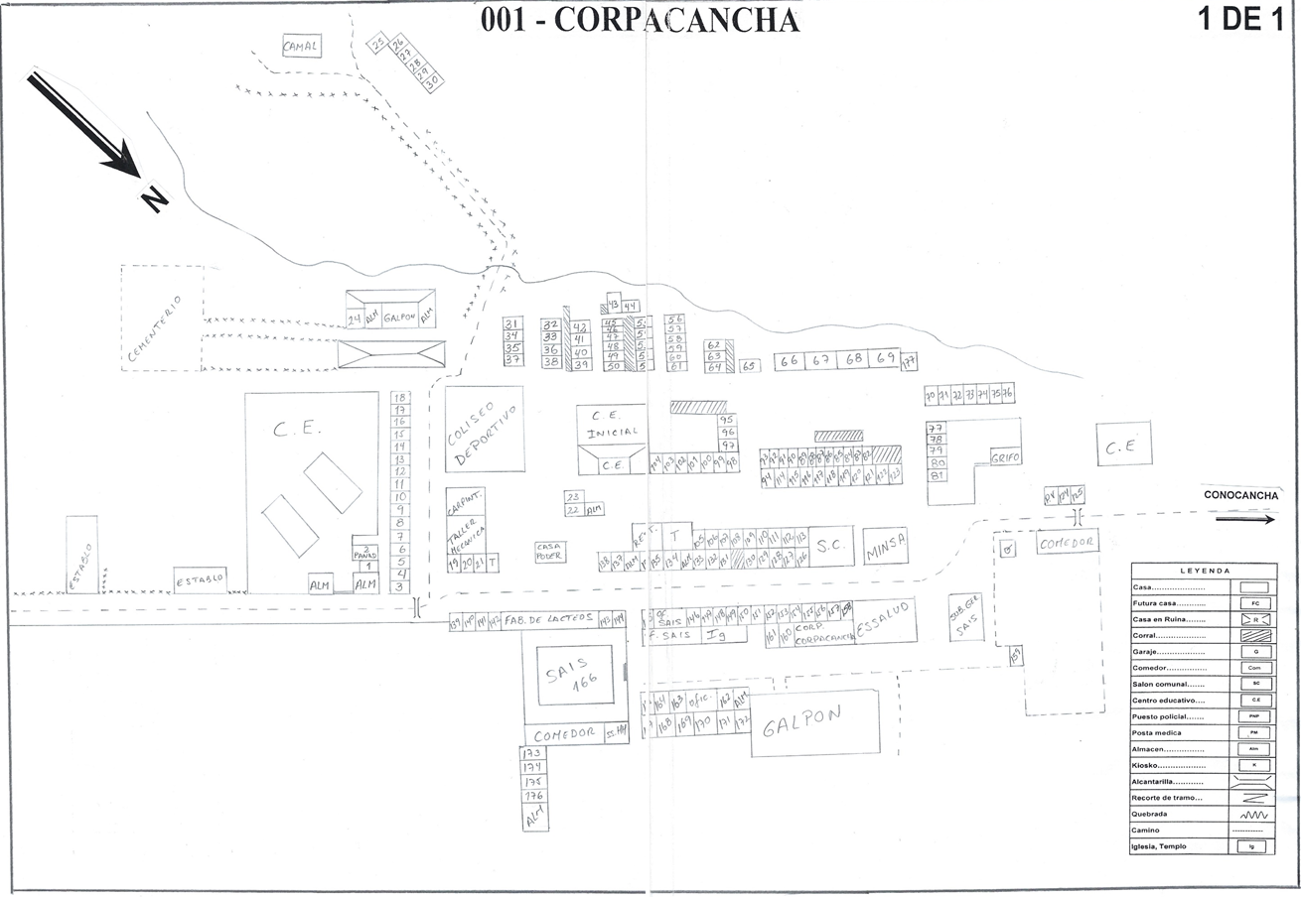
\includegraphics[width=0.5\textwidth]{imagenes/corpacancha_mapa.png} %,angle=180
\caption{Mapa urbano del centro poblado de Corpacancha (Junín, Perú)}
\end{figure}

\newpage

\section{Cuadro de operacionalización de variables}
\begin{table}[htbp]
  \centering
  \caption{Cuadro de operalización de variables}
  \vspace{0.5cm}
    \begin{tabular}{|p{6.355em}|p{11.93em}|p{5.145em}|p{11.215em}|}
    \toprule
    Variable & Definición Conceptual & Tipo  & Valores \\
    \midrule
    Distancia & Distancia en metros desde la casa de un individuo al centro de EsSalud & Continua & Número real mayor a 0 \\
    \midrule
    Prevalencia & Proporción de individuos que presentan la enfermedad & Continua & Número real comprendido entre 0 y 1 \\
    \midrule
    Sexo  & Sexo del individuo & Nominal & 0: Femenino\newline{}1: Másculino \\
    \midrule
    Edad  & Tiempo de vida en años del individuo & Discreta & Número entero mayor o igual a 0 \\
    \midrule
    Rango de edad & Tiempo de vida en años del individuo agrupado en rangos & Ordinal & 1: Menores de 15 años\newline{}2: De 16 a 30 años\newline{}3: De 31 a 40 años\newline{}4: De 41 a 50 años\newline{}5: De 51 a 65 años\newline{}6: De 66 años a más \\
    \bottomrule
    \end{tabular}%
  \label{tab:addlabel}%
\end{table}%



\section{Matriz de consistencia}
En la siguiente página, en la Tabla \ref{matcons}, encontramos la matriz de consistencia del estudio
\newpage
\begin{landscape}

\begin{table}[htbp]
  \centering
  \caption{Matriz de consistencia}\label{matcons}
  \vspace{0.5cm}
    \begin{tabular}{|p{11.07em}|p{11.07em}|r|r|p{11.07em}|}
    \toprule
    \textbf{Problema} & \textbf{Objetivos} & \multicolumn{1}{p{11.07em}|}{\textbf{Hipótesis}} & \multicolumn{1}{p{11.07em}|}{\textbf{Variables e Indicadores}} & \textbf{Metodología} \\
    \midrule
    \textbf{Problema General} & \textbf{Objetivo General} & \multicolumn{1}{p{11.07em}|}{\textbf{Hipótesis General}} & \multicolumn{1}{p{11.07em}|}{\textbf{Variable dependiente}} & \textbf{Tipo de Investigación} \\
    ¿Se puede emplear un método de estimación de prevalencia considerando la distribución espacial para reducir el sesgo del muestreo? & Estudiar un método de estimación de prevalencia considerando la distribución espacial para reducir el sesgo del muestreo & \multicolumn{1}{p{11.07em}|}{El método planteado estima la prevalencia de forma insesgada} & \multicolumn{1}{p{11.07em}|}{Prevalencia: Porcentaje de individuos que presentan la enfermedad} & Básica. \\
    \textbf{Problemas Específicos} & \textbf{Objetivos Específicos} & \multicolumn{1}{p{11.07em}|}{\textbf{Hipótesis Específica}} & \multicolumn{1}{p{11.07em}|}{\textbf{Variable independiente}} & \textbf{Tipo de Investigación} \\
    ¿Cómo se diferencian los resultados obtenidos de las estimaciones de la prevalencia mediante el método clásico y el error de estimación del método propuesto? & Comparar los resultados obtenidos de las estimaciones de la prevalencia por el método tradicional y el método propuesto & \multicolumn{1}{p{11.07em}|}{El método planteado presenta un menor Error Cuadrático Medio en la estimación de la prevalencia que el método tradicional.} & \multicolumn{1}{p{11.07em}|}{Ubicación de la vivienda del individuo} & Observacional. \\
    ¿Cuál es el método adecuado de acuerdo a las condiciones de la investigación? & Determinar el método adecuado de acuerdo a las condiciones de la investigación. & \multicolumn{1}{p{11.07em}|}{El método planteado es el adecuado para la situación que se está observando} & \multicolumn{1}{p{11.07em}|}{Presencia de la enfermedad en el individuo} & A fin de comparar los métodos antes de aplicarlos en la data real, se simularán escenario tomando en consideración diferentes condiciones. \\
    ¿De cuánta es la prevalencia de la hidatidosis humana en el centro poblado de Corpacancha mediante el método propuesto y de cuanta sería en un centro poblado diferente? & Estimar la prevalencia de la hidatidosis humana en el centro poblado de Corpacancha y en un centro poblado diferente mediante el método propuesto. &       &   Covariables epidemiológicas    & La información del caso a tratar proviene de dos campañas médicas realizadas en la comunidad. \\
    \bottomrule
    \end{tabular}
  
\end{table}%

\end{landscape}

%----------------------------------------------------------------------------------------
%	ANÁLISIS Y RESULTADOS
%----------------------------------------------------------------------------------------
\chapter{ANÁLISIS Y RESULTADOS}

\section{Análisis Exploratorio}
El centro poblado de Corpacancha cuenta con 177 casas, de las cuales 105 (59.3\%) están habitadas. Del censo realizado en 2018, se conoce que la población es de un total de 309 habitantes; de los cuales 141 (45.6\%) participaron en la campaña de salud. Tras haber realizado la limpieza correspondiente a los datos de la muestra proveniente del estudio VIRSEL, se conoce que la Hidatidosis Humana en el Centro poblado de Corpacancha tiene una prevalencia del 0.241 ($\pm$ 0.054 IC$_{95\%}$). Este estudio contó con una potencia estadística del 22.1 por ciento. La segunda campaña realizada junto al censo permitió aumentar la cobertura a un total de 196 participantes (63.4\%). Como resultado, la prevalencia disminuyó a 0.235 ($\pm$ 0.036 IC$_{95\%}$); indicando que la prevalencia del primer estudio se encontraba sobreestimada. Este estudio contó con una potencia estadística del 28.8 por ciento.

\newpage

\begin{figure}[h]\label{houses}
	\begin{center}
		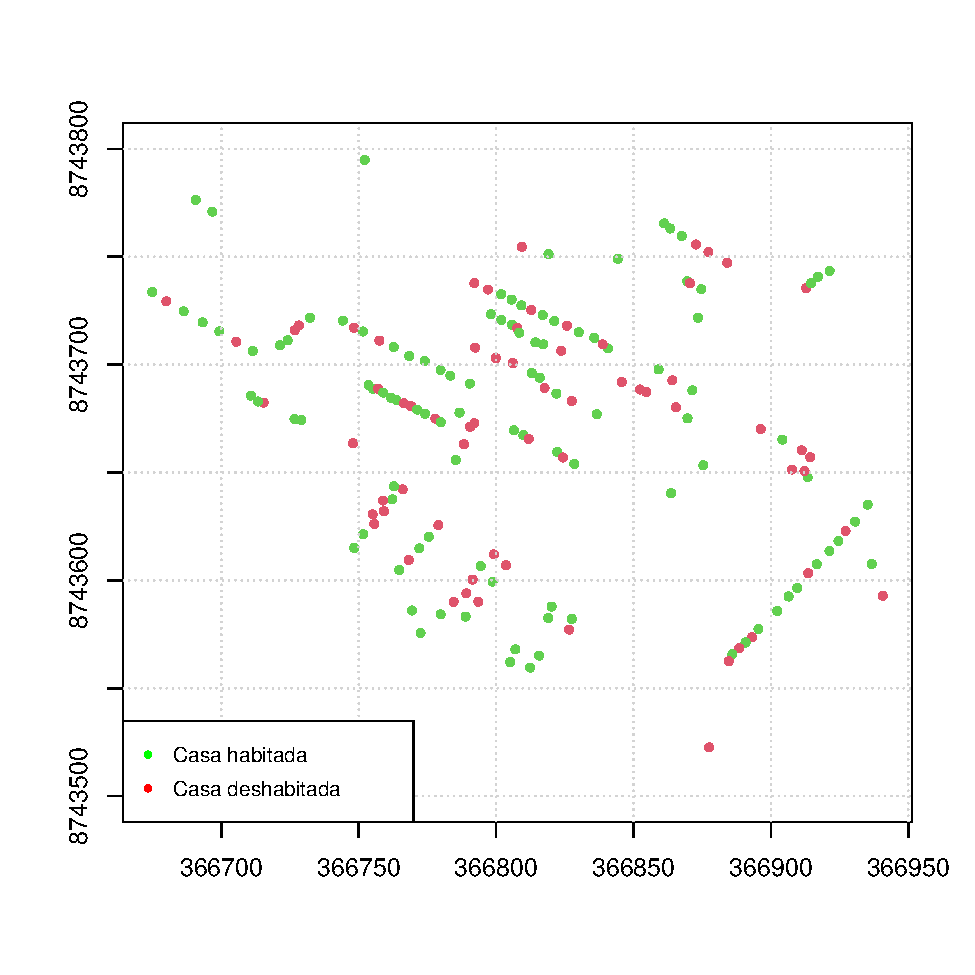
\includegraphics[width=0.85\textwidth]{graficos/houses.pdf}
	\end{center}
	\caption{Distribución en el espacio de las casas en el centro poblado de Corpacancha.}
\end{figure}

\newpage

\begin{figure}[h]\label{houses_participation}
	\begin{center}
		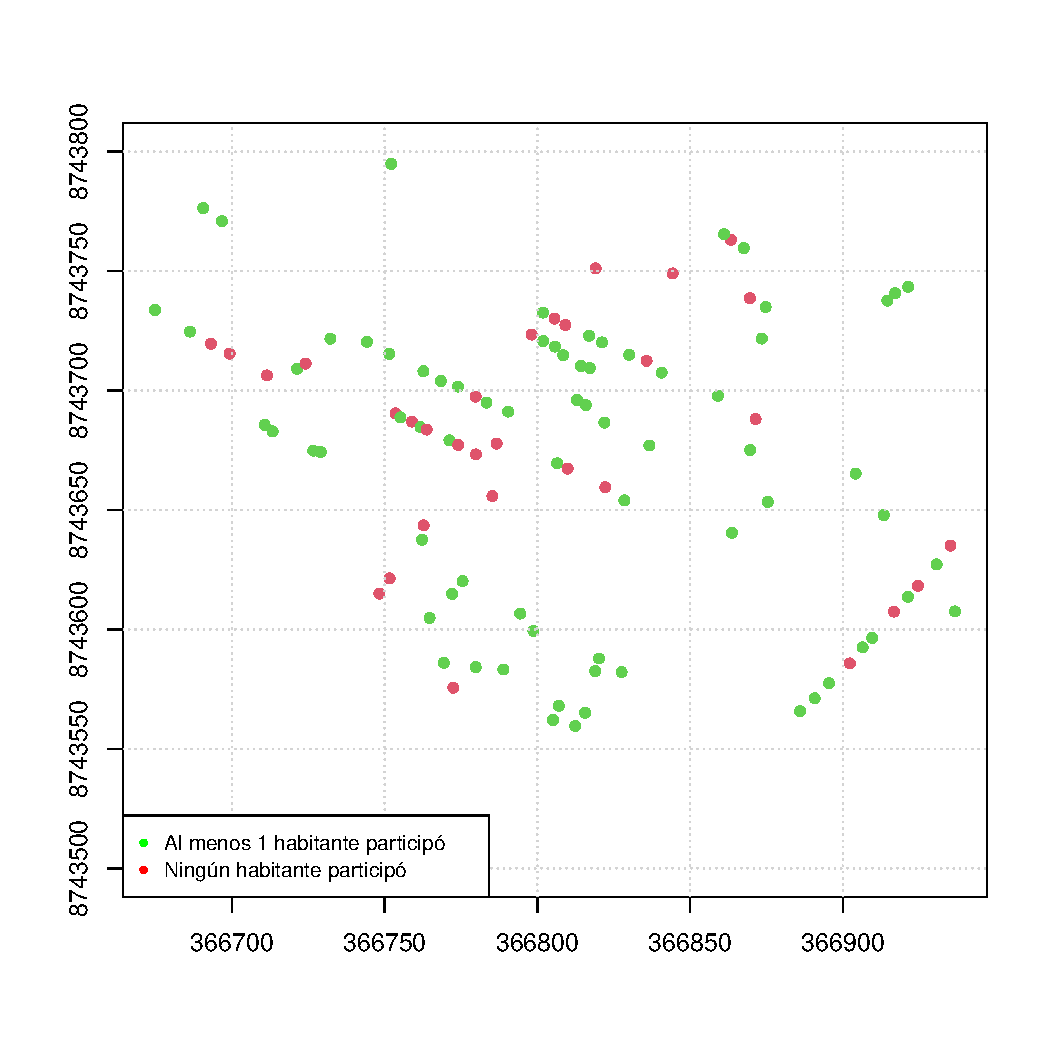
\includegraphics[width=0.85\textwidth]{graficos/houses_participation.pdf}
	\end{center}
	\caption{Distribución en el espacio de las casas habitadas en el centro poblado de Corpacancha.}
\end{figure}

\newpage

\begin{figure}[h]\label{houses_hidatidosis}
	\begin{center}
		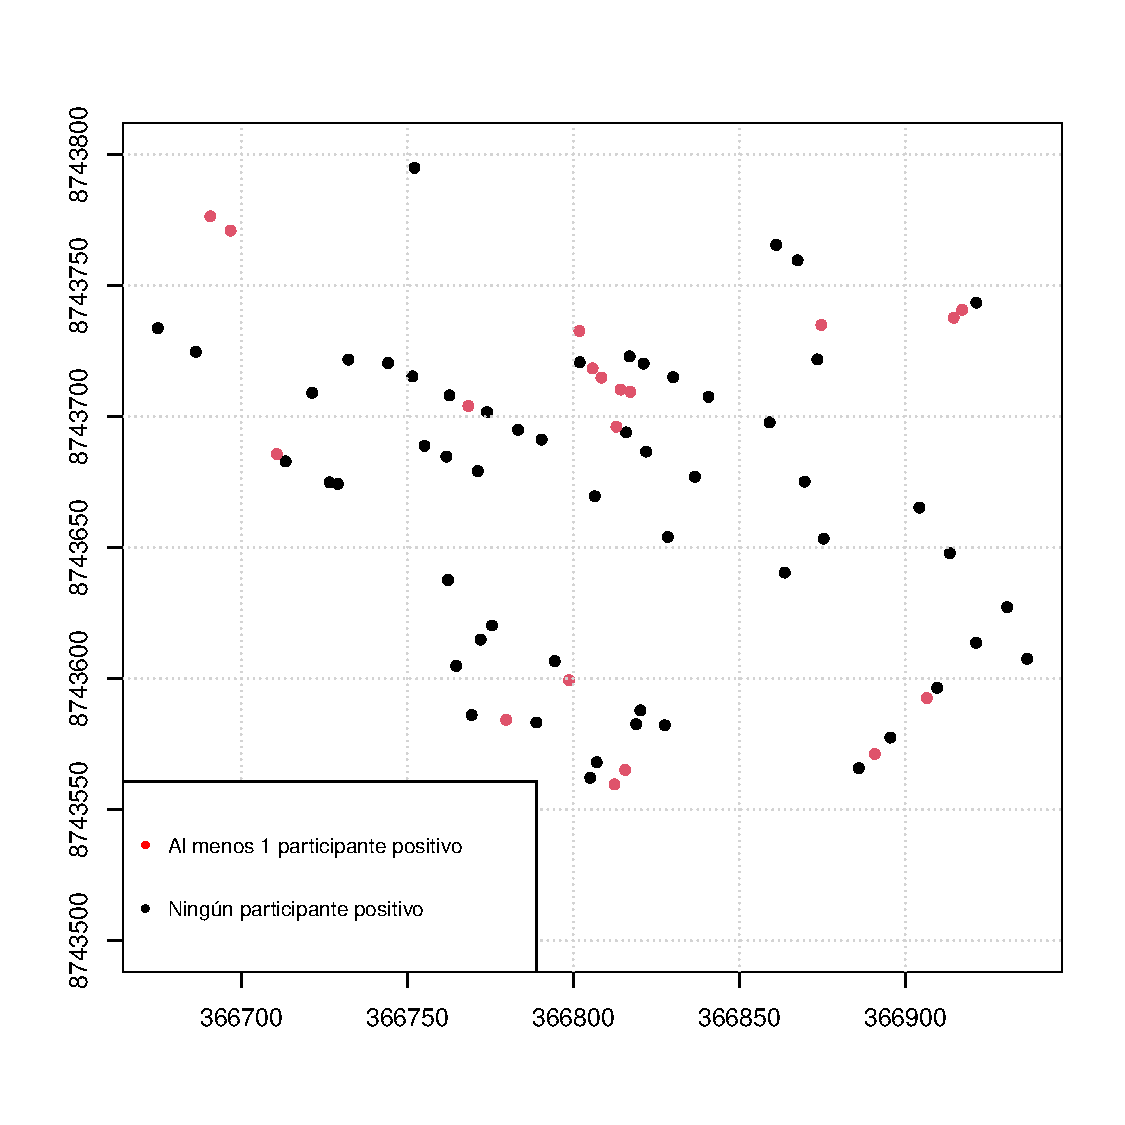
\includegraphics[width=0.85\textwidth]{graficos/houses_hidatidosis.pdf}
	\end{center}
	\caption{Distribución de las casas con al menos un habitante que haya participado en la campaña realizada en el centro poblado de Corpacancha.}
\end{figure}

\newpage

\begin{figure}[h]\label{prevalence_samplesize}
	\begin{center}
		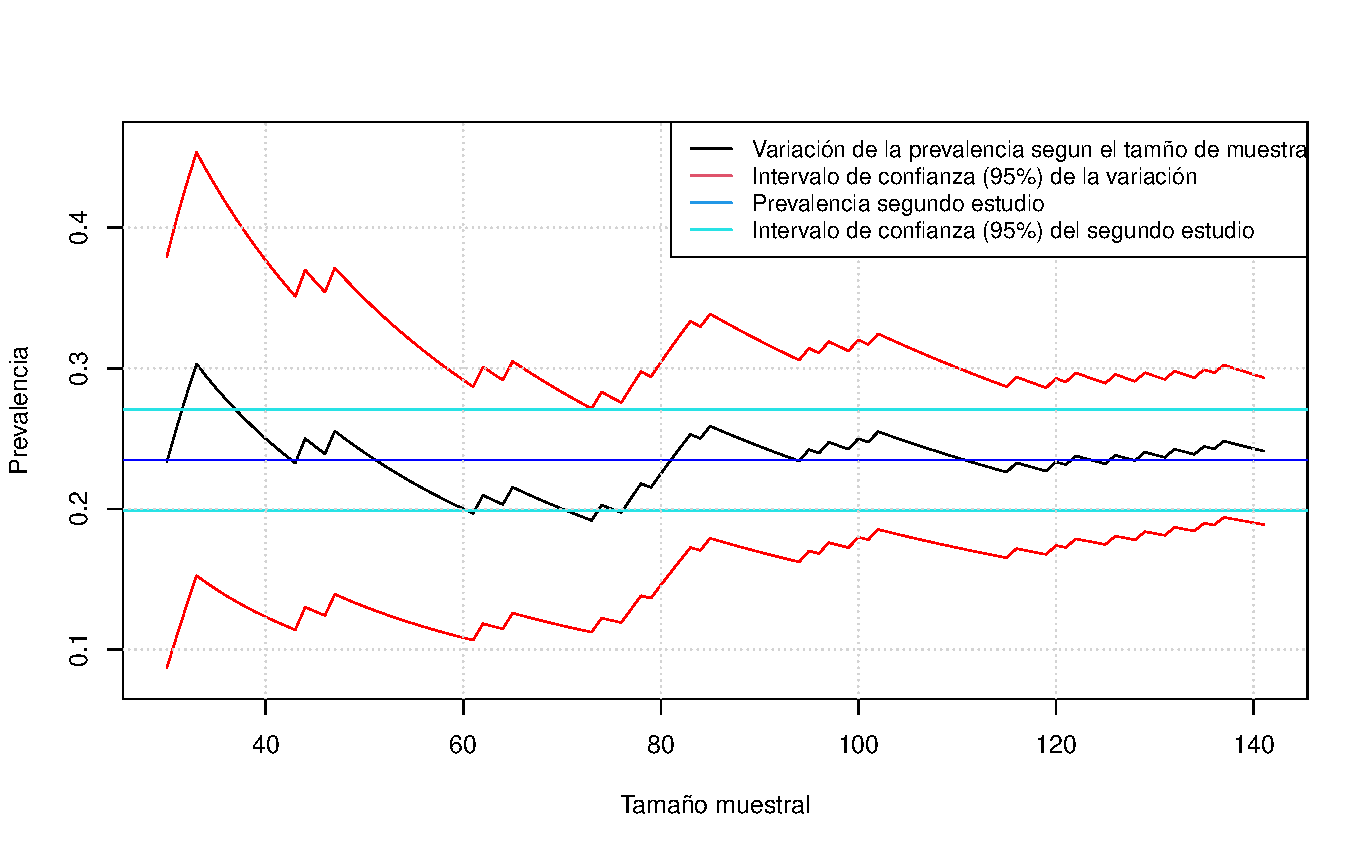
\includegraphics[width=1\textwidth]{graficos/prevalence_samplesize.pdf}
	\end{center}
	\caption{Prevalencia de Hidatidosis Humana en Corpacancha.}
\end{figure}

\newpage

\subsection{Análisis de los factores de riesgo}
De la base de datos, se seleccionaron como covariables a los factores de riesgo determinados en estudios anteriores en la región~\cite{santivanez2010factores}. El resumen de esta información, tanto univariado, como bivariado respecto a la prevalencia, se puede encontrar en las tablas \ref{DescripFactRiesPrev} y \ref{PrevFact}. En esta segunda tabla se observaron diferencias que fueron necesarias estudiar.

\begin{table}[h]
	\centering
	\caption{Factores de riesgo y prevalencia (n=141).}\label{DescripFactRiesPrev}
	\begin{tabular}{llll}
		\toprule
		\textbf{Características} &       & \multicolumn{1}{c}{\textbf{n}} & \multicolumn{1}{c}{\textbf{\%}} \\
		\midrule
		\multicolumn{2}{l}{Sexo} &       &  \\
		& Femenino & \multicolumn{1}{c}{83} & \multicolumn{1}{c}{58.9} \\
		& Masculino & \multicolumn{1}{c}{58} & \multicolumn{1}{c}{41.1} \\
		\midrule
		\multicolumn{2}{l}{Edad *} & \multicolumn{2}{c}{33.27 ($\pm$ 3.19)} \\
		\midrule
		\multicolumn{2}{l}{Nùmero de perros} &       &  \\
		& 0     & \multicolumn{1}{c}{95} & \multicolumn{1}{c}{67.4} \\
		& 1     & \multicolumn{1}{c}{15} & \multicolumn{1}{c}{10.6} \\
		& 2     & \multicolumn{1}{c}{17} & \multicolumn{1}{c}{12.1} \\
		& 3     & \multicolumn{1}{c}{11} & \multicolumn{1}{c}{7.8} \\
		& 4     & \multicolumn{1}{c}{3} & \multicolumn{1}{c}{2.1} \\
		\midrule
		\multicolumn{2}{l}{Prevalencia**} & \multicolumn{2}{c}{0.241 ($\pm$ 0.054)} \\
		\midrule
		\multicolumn{4}{l}{* Promedio (IC 95\%)} \\
		\multicolumn{4}{l}{** Proporción (IC 95\%)} \\
	\end{tabular}% 
\end{table}%

\newpage

\begin{table}[h]
	\centering
	\caption{Factores de riesgo por resultado de la campaña (n=141).}\label{PrevFact}
	\begin{tabular}{llll}
		\toprule
		\multicolumn{2}{l}{\textbf{Factor de riesgo}} & \multicolumn{1}{c}{\textbf{Positivo}} & \multicolumn{1}{c}{\textbf{Negativo}} \\
		\midrule
		\multicolumn{2}{l}{Sexo} &       &  \\
		& \multicolumn{1}{c}{Male} & \multicolumn{1}{c}{16 (27.6\%)} & \multicolumn{1}{c}{42 (72.4\%)} \\
		& \multicolumn{1}{c}{Female} & \multicolumn{1}{c}{18 (21.7\%)} & \multicolumn{1}{c}{65 (78.3\%)} \\
		\midrule
		\multicolumn{2}{l}{Edad*} & \multicolumn{1}{c}{36.1 $\pm$ 6.7} & \multicolumn{1}{c}{32.4 $\pm$ 3.6} \\
		\midrule
		\multicolumn{2}{l}{Número de perros} &       &  \\
		& \multicolumn{1}{c}{0} & \multicolumn{1}{c}{21 (22.1\%)} & \multicolumn{1}{c}{74 (77.9\%)} \\
		& \multicolumn{1}{c}{1} & \multicolumn{1}{c}{2 (13.3\%)} & \multicolumn{1}{c}{13 (86.7\%)} \\
		& \multicolumn{1}{c}{2} & \multicolumn{1}{c}{3 (17.6\%)} & \multicolumn{1}{c}{14 (82.4\%)} \\
		& \multicolumn{1}{c}{3} & \multicolumn{1}{c}{7 (63.6\%)} & \multicolumn{1}{c}{4 (36.4\%)} \\
		& \multicolumn{1}{c}{4} & \multicolumn{1}{c}{1 (33.3\%)} & \multicolumn{1}{c}{2 (66.7\%)} \\
		\midrule
		\multicolumn{4}{l}{* Media por resultado} \\
	\end{tabular}%
\end{table}%


\subsubsection{Sexo}
En la tabla \ref{PrevFact}, se observó que hay una diferencia en la prevalencia por sexo de la persona. Pese a esto, la diferencia encontrada no era significativa debido a la superposición de los invervalos de confianza de cada una (Fig. \ref{bar_sexoprevalencia}).

\begin{figure}[h]
	\centering
	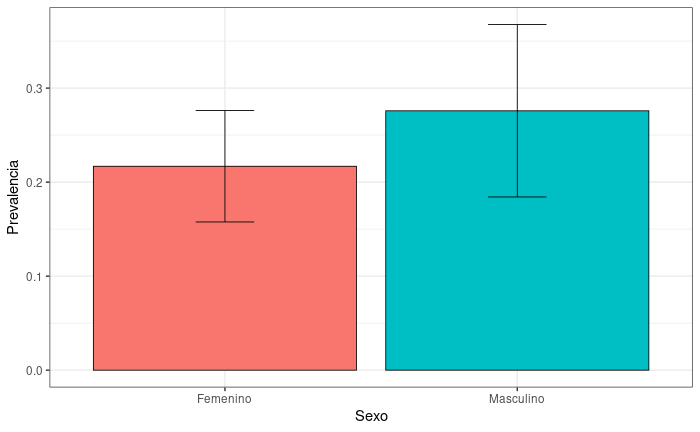
\includegraphics[width=0.7\textwidth]{graficos/sexoprevalencia.png}
	\caption{Prevalencia e intervalo de confianza por sexo.}
	\label{bar_sexoprevalencia}
\end{figure}

\newpage

Ajustando un modelo lineal generalizado entre el sexo y la prevalencia de hidatidosis, se observó que la posibilidad de tener hidatidosis siendo hombre es 1.38 veces la posibilidad siendo mujer (Tabla \ref{or_sexo}). Pese a que los resultados no son significativos, esto no descarta que se considere como factor de riesgo debido a que el p-valor se encuentra relacionado con la potencia estadística que tuvo la muestra~\cite{ellis2010essential}.


\begin{table}[h]
	\centering
	\caption{Odd Ratio de la variable sexo}
	\label{or_sexo}
	\begin{tabular}{lccc}
		\hline
		& OR*   & IC 95\%           & p-valor \\ \hline
		\multicolumn{1}{c}{Sexo = Masculino}  & 1.38  & [0.63; 3.00] & 0.421   \\ \hline
		\multicolumn{4}{l}{*obtenido al ajustar un modelo lineal generalizado}
	\end{tabular}
\end{table}

\subsubsection{Edad}
En la tabla \ref{PrevFact}, se observó que hay una diferencia en la edad promedio entre el grupo positivo a la enfermedad y el grupo negativo a la enfermedad. No obstante, esta diferencia resultó ser no significativa pues sus intervalor de confianza se superponen. Ajustando un modelo lineal generalizado entre el edad y la prevalencia de hidatidosis, se observó que la posibilidad de tener hidatidosis se incrementaba 1.01 veces con cada año de edad (Tabla \ref{or_edad}). Pese a que los resultados no son significativos, esto no descarta que se considere como factor de riesgo. Esto debido a que el p-valor se encuentra relacionado con la potencia estadística que tuvo la muestra~\cite{ellis2010essential}.

\begin{table}[h]
	\centering
	\caption{Odd Ratio de la variable edad}
	\label{or_edad}
	\begin{tabular}{lccc}
		\hline
		& OR*   & IC 95\%          & p-valor \\ \hline
		\multicolumn{1}{c}{Edad}  & 1.01  & [0.99; 1.03] & 0.334   \\ \hline
		\multicolumn{4}{l}{*obtenido al ajustar un modelo lineal generalizado}
	\end{tabular}
\end{table}

\newpage

\subsubsection{Número de perros}
En la tabla \ref{PrevFact}, se observó que hay una diferencia en la prevalencia por el número de perros que se tienen. La diferencia encontrada era significativa cuando se dicotomizaba la variable del número de perros. Esto debido a la no superposición de los invervalos de confianza de cada una (Fig. \ref{fig:bar_perrosprevalencia}). Ajustando un modelo lineal generalizado entre el número de perros y la prevalencia de hidatidosis, se observó que la posibilidad de tener hidatidosis teniendo menos de tres perros es 0.19 veces la posibilidad teniendo al menos tres perros (Tabla \ref{or_sexo}). Esto determinó que en adeltante, la variable número de perros sea tomada como cualitativa con dos categoría: menos de tres perros y al menos tres perros.

\begin{figure}[h]
	\centering
	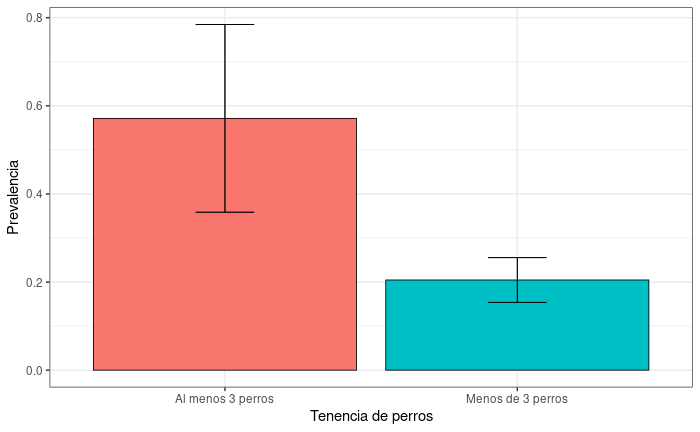
\includegraphics[width=0.7\textwidth]{graficos/perrosprevalencia.png}
	\caption{Prevalencia e intervalo de confianza por tenencia de perros.}
	\label{fig:bar_perrosprevalencia}
\end{figure}

\begin{table}[h]
	\centering
	\caption{Odd Ratio de la variable perro}
	\label{or_perros}
	\begin{tabular}{cccc}
		\hline
		\multicolumn{1}{l}{}          & OR*     & IC 95\%              & p-valor   \\ \hline
		Perros = 1                    & 0.54    & [0.08; 2.17]     & 0.443     \\
		Perros = 2                    & 0.76    & [0.16; 2.59]     & 0.681     \\
		Perros = 3                    & 6.17    & [1.70; 25.49]    & 0.007     \\
		Perros = 4                    & 1.76    & [0.08; 19.28]    & 0.650     \\ \hline
		Perros = Menos de 3 perros    & 0.19    & [0.06; 0.60]     & 0.005     \\ \hline
		\multicolumn{4}{l}{*obtenido al ajustar un modelo lineal generalizado}
	\end{tabular}
\end{table}

\newpage
\subsection{Análisis de la intensidad}
Se observó que la población se concentra al sureste del centro de salud en el que se hizo la campaña (Fig. \ref{intensity_population}). Se encontró un comportamiento similar en los habitantes que participaron en la campaña (Fig. \ref{intensity_sample}). No obstante, era necesario observar si la razón de las intensidades se mantiene constante en el espacio. En la figura \ref{risk_to_sampling} se observó que el riesgo de participar en la muestra no es constante en el área; especialmente en la zona noroeste. Esto planteó la existencia  de un posible sesgo espacial.

\begin{figure}[h]
	\centering
	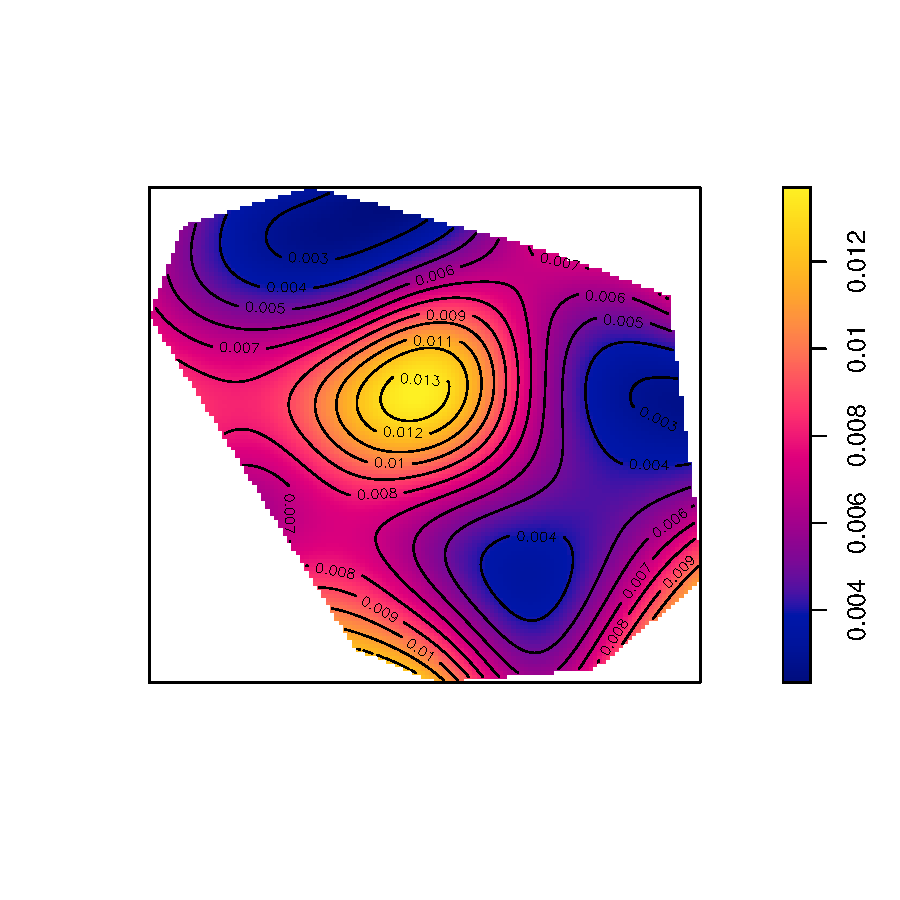
\includegraphics[width=0.9\textwidth]{graficos/intensity_population.pdf}
	\caption{Intensidad poblacional} \label{intensity_population}
\end{figure}

\newpage

\begin{figure}[h]
	\centering
	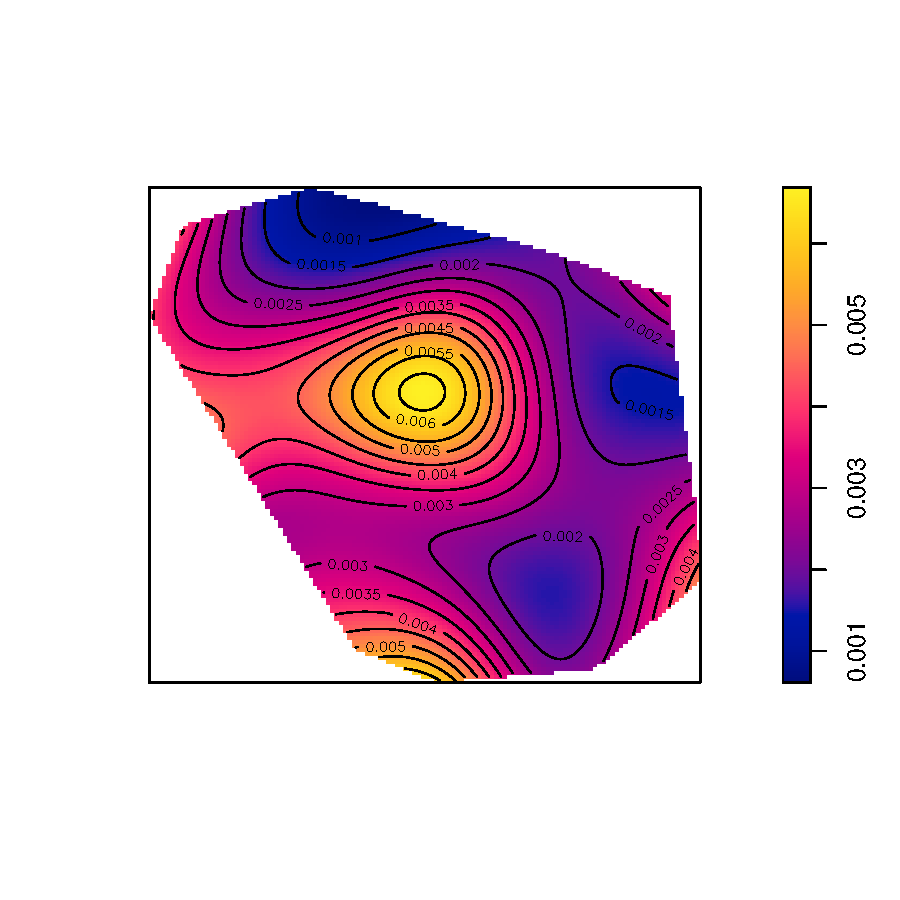
\includegraphics[width=0.9\textwidth]{graficos/intensity_sample.pdf}
	\caption{Intensidad muestral} \label{intensity_sample}
\end{figure}

\newpage

\begin{figure}[h]
	\centering
	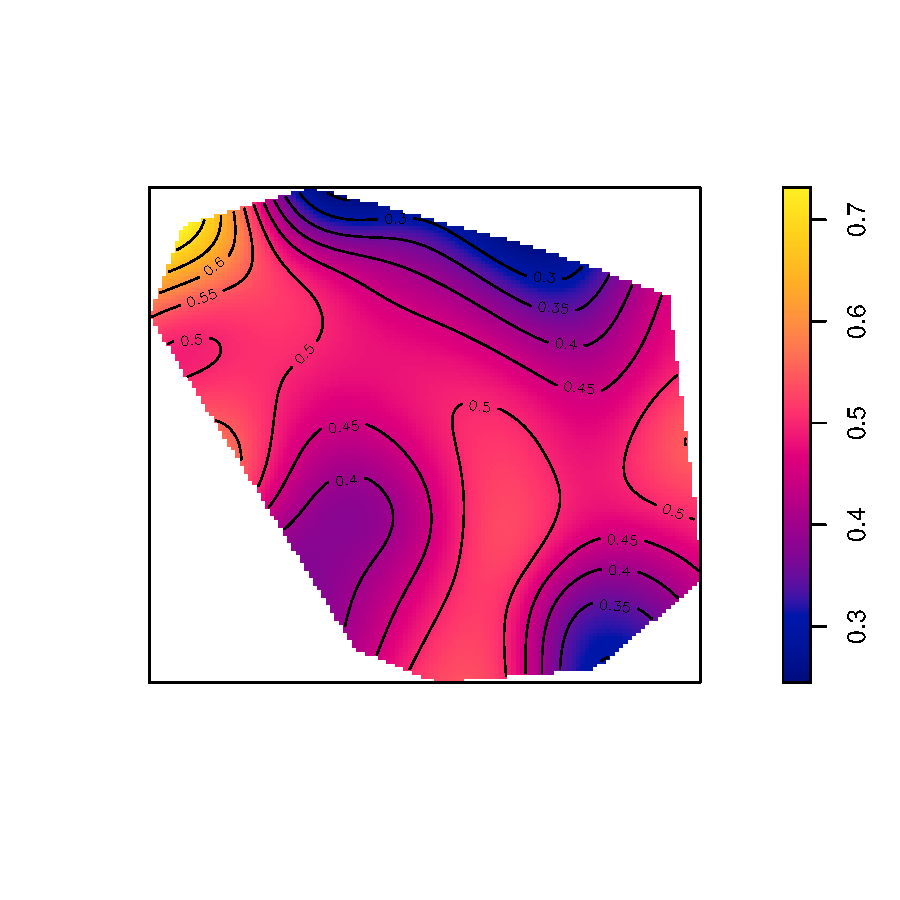
\includegraphics[width=0.9\textwidth]{graficos/risk_to_sampling.pdf}
	\caption{Riesgo de participar en la muestra}
	\label{risk_to_sampling}
\end{figure}

\newpage

Lo visto en la Figura \ref{risk_to_sampling} indicó la necesidad de corregir el riesgo de tener la enfermedad a nivel espacial (Fig.~\ref{risk_to_disease}).
\begin{figure}[h]
	\centering
	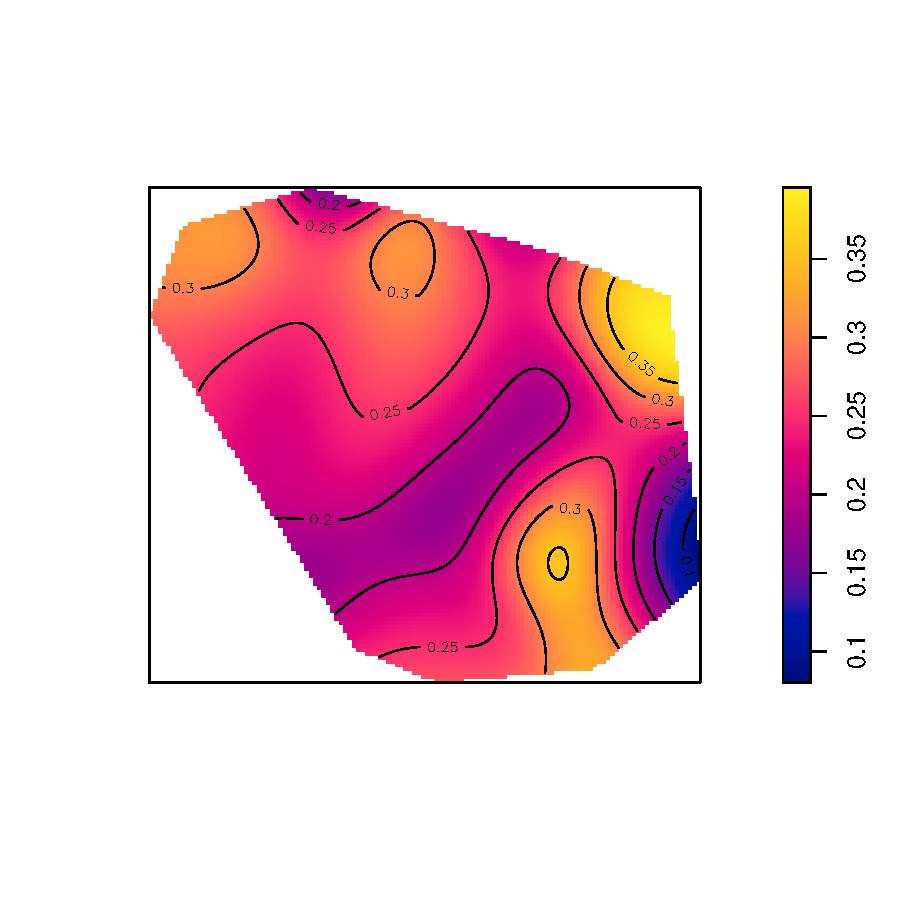
\includegraphics[width=0.9\textwidth]{graficos/risk_to_disease.pdf}
	\caption{Riesgo de tener la enfermedad}
	\label{risk_to_disease}
\end{figure}

\newpage

\section{Simulaciones}

Cada una de las simulaciones y sus resultados fueron evaluados por escenario (Tabla \ref{simu_resul}, Figura \ref{simu_01-09} y Figura \ref{simu_10-18}). Si bien el ECM($\tilde{\theta}$) resultó ser mayor al ECM($\hat{\theta}$) en cada escenario, también se observó que en su mayoría estos superaron el 15\% de éxito; o sea, que en 13 de 18 escenarios, al menos el 15\% de las simulaciones, la estimación de la prevalencia por medio del método presentado tenía un valor más cercano al real que la estimación por el método convencional. Este comportamiento también se observó en los escenarios con las caraterísticas más similares a la data real, a nivel de cobertura y tamaño poblacional. Pese a esto, las curvas de densidad en cada escenario presentaron notorias diferencias entre si.


\begin{table}[h]
	\centering
	\caption{Resultados de la simulación}
	\label{simu_resul}
	\begin{tabular}{cccccccc}
		\hline
		Escenario & m   & Éxitos (\%) & $\hat{n}$ & Cobertura & Prevalencia* & ECM($\hat{\theta}$) & ECM($\tilde{\theta}$) \\ \hline
		1         & 506 & 33.20      & 249        & 34.67     & 0.252       & 0.0014 & 0.0037 \\
		2         & 510 & 23.92      & 249        & 44.95     & 0.250       & 0.0009 & 0.0049 \\
		3         & 509 & 21.61      & 250        & 54.86     & 0.251       & 0.0006 & 0.0053 \\
		4         & 510 & 23.53      & 349        & 35.09     & 0.251       & 0.0010 & 0.0066 \\
		5         & 510 & 15.69      & 350        & 44.94     & 0.249       & 0.0007 & 0.0080 \\
		6         & 510 & 10.78      & 350        & 54.86     & 0.252       & 0.0004 & 0.0087 \\
		7         & 510 & 14.12      & 451        & 35.09     & 0.249       & 0.0007 & 0.0118 \\
		8         & 510 & 8.43       & 450        & 45.08     & 0.251       & 0.0005 & 0.0108 \\
		9         & 510 & 6.47       & 450        & 55.21     & 0.251       & 0.0003 & 0.0098 \\
		10        & 509 & 15.52      & 247        & 34.28     & 0.241       & 0.0040 & 0.0271 \\
		11        & 499 & 15.83      & 246        & 44.38     & 0.243       & 0.0009 & 0.0153 \\
		12        & 510 & 16.86      & 247        & 55.41     & 0.242       & 0.0007 & 0.0088 \\
		13        & 503 & 20.68      & 344        & 34.50     & 0.242       & 0.0033 & 0.0259 \\
		14        & 506 & 16.60      & 342        & 44.20     & 0.243       & 0.0007 & 0.0127 \\
		15        & 509 & 15.52      & 343        & 55.47     & 0.243       & 0.0005 & 0.0080 \\
		16        & 510 & 21.96      & 440        & 34.40     & 0.241       & 0.0034 & 0.0236 \\
		17        & 510 & 15.69      & 440        & 44.16     & 0.242       & 0.0005 & 0.0124 \\
		18        & 510 & 14.51      & 440        & 55.36     & 0.242       & 0.0004 & 0.0088 \\ \hline
		\multicolumn{8}{l}{m: Número de simulaciones por escenario}                           \\
		\multicolumn{8}{l}{n: Número promedio de personas por escenario}                      \\
		\multicolumn{8}{l}{Cobertura*: Cobertura de muestreo promedio por escenario}          \\
		\multicolumn{8}{l}{Prevalencia*: Prevalencia promedio por escenario}                  \\ \hline
	\end{tabular}
\end{table}

\newpage

\begin{figure}[h] 
	\centering
	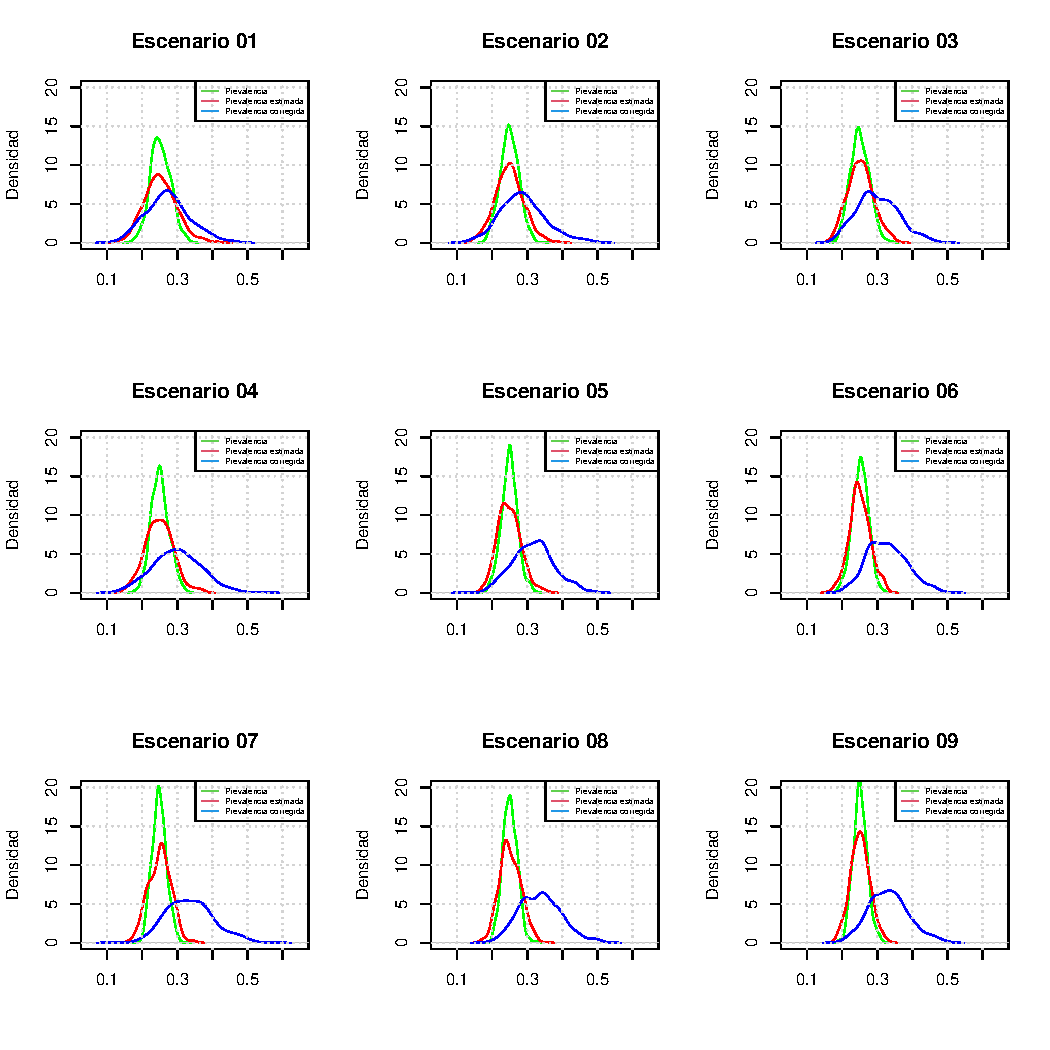
\includegraphics[width=1\textwidth]{graficos/simu_01-09.pdf}
	\caption{Densidad del parámetro de los escenarios 1 al 9} \label{simu_01-09}
\end{figure}

\newpage

\begin{figure}[h] 
	\centering
	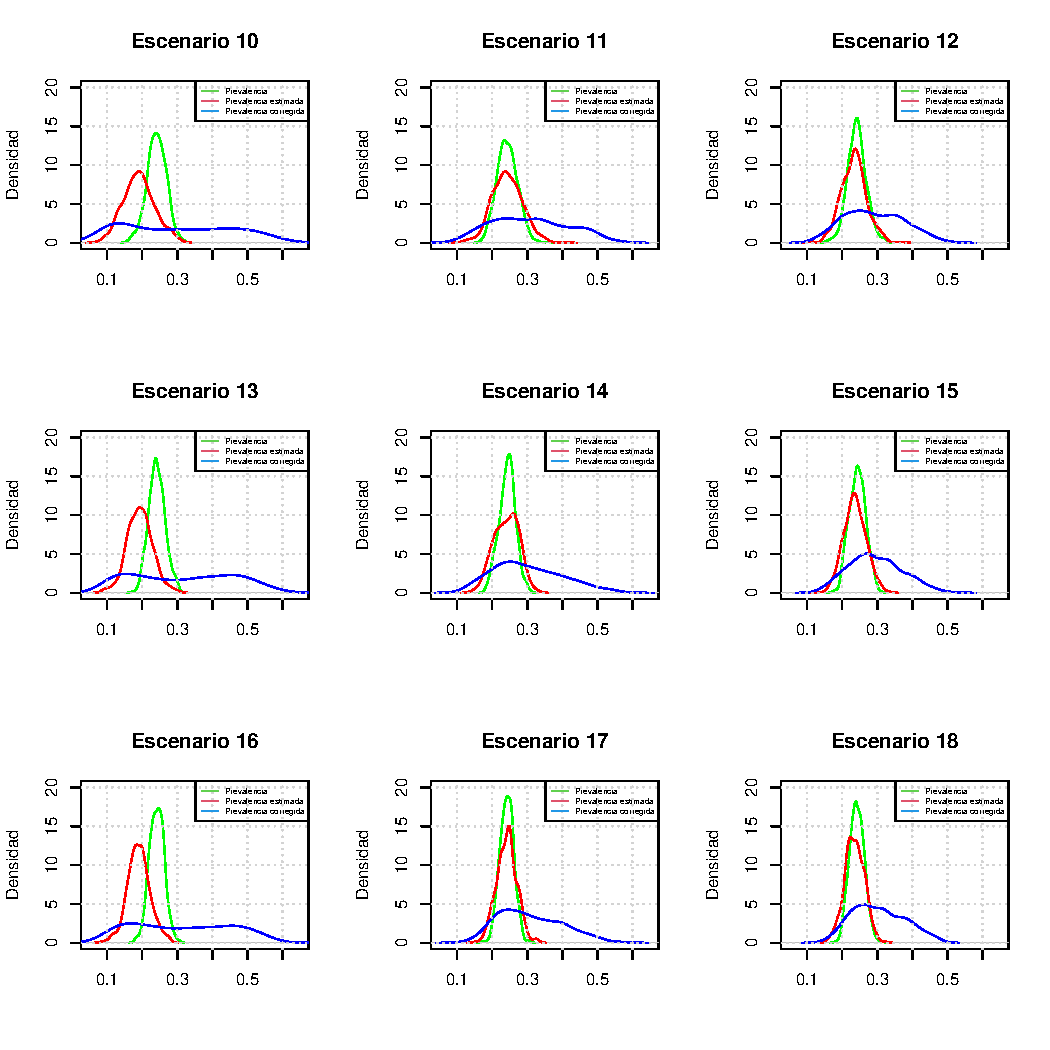
\includegraphics[width=1\textwidth]{graficos/simu_10-18.pdf}
	\caption{Densidad del parámetro de los escenarios 10 al 18} \label{simu_10-18}
\end{figure}


\newpage

\section{Modelamiento}
\subsection{Intensidad}
\label{seccion_intensidad}
En la estimación de la función de intensidad para la población y la muestra, los modelos se ajustaron con 14 y 16 funciones de base, respectivamente, en base a sus residuales (Véase Fig.~\ref{intensity_population_residuals} y~\ref{intensity_sample_residuals} )

\subsubsection{Homogeneidad de riesgo}

En base al algoritmo \ref{validaHipo}, se determinó que el riesgo al ser seleccionado es no homogéneo, debido a que en más de una observación, el cociente entre las dos intensidades no se ha encontrado en el intervalo de confianza correspondiente. Este resultado confirmó lo visto en la Figura \ref{risk_to_sampling}.

%\begin{figure}[h] 
%	\centering
%	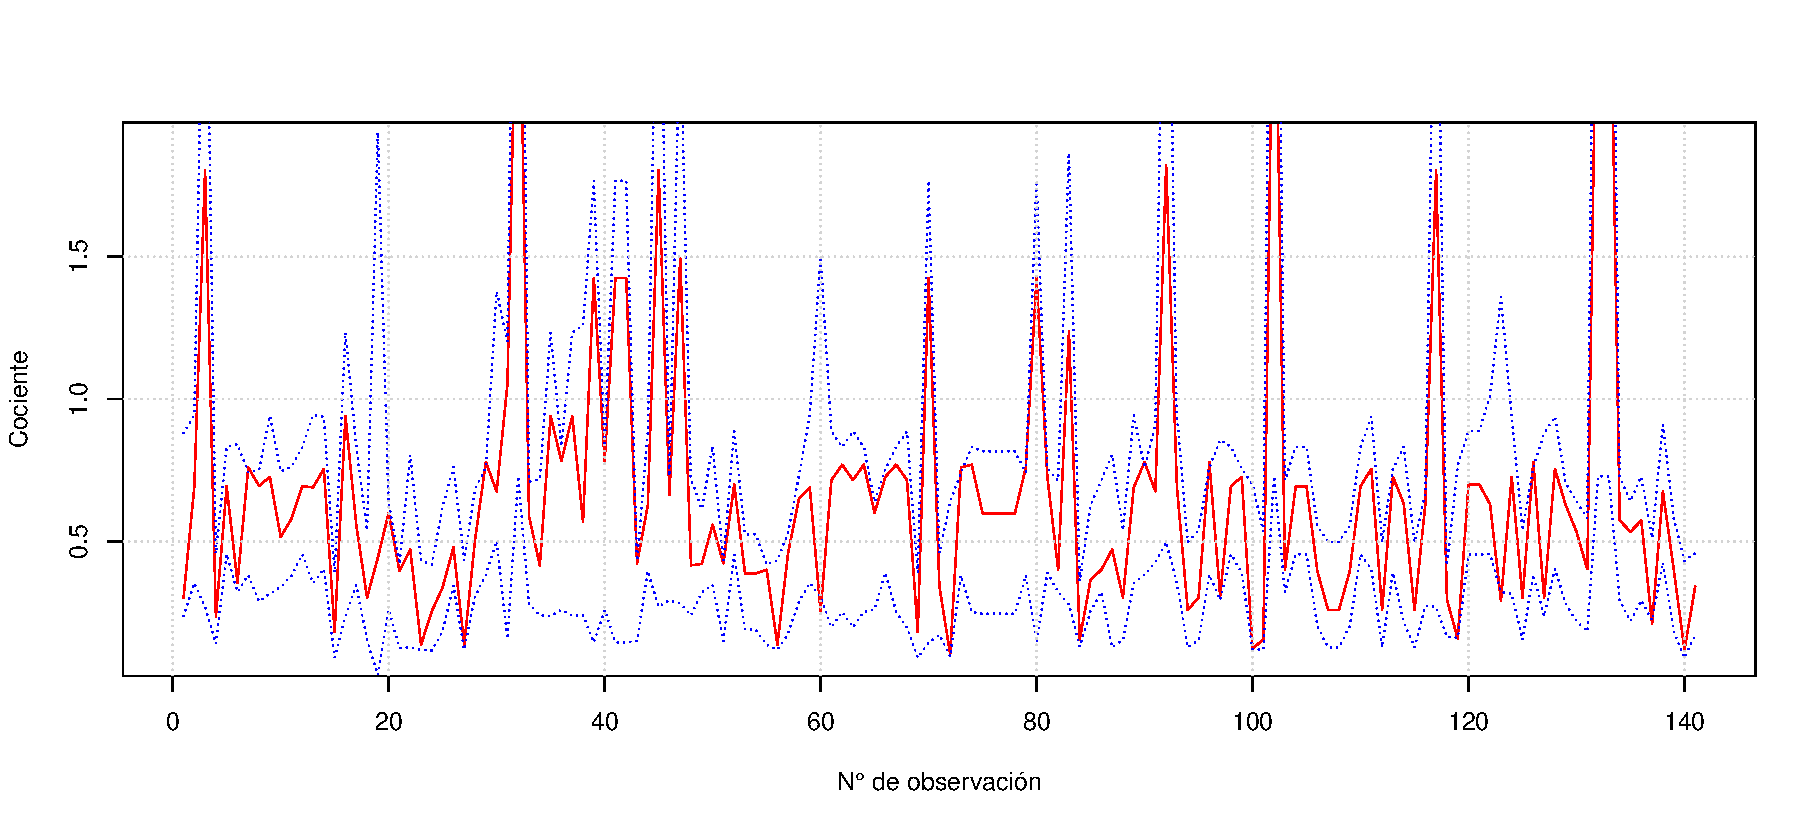
\includegraphics[width=1\textwidth]{graficos/montecarlo.pdf}
%	\caption{Cociente de intensidades} \label{montecarlo}
%\end{figure}


\newpage

\begin{figure}[h] 
	\centering
	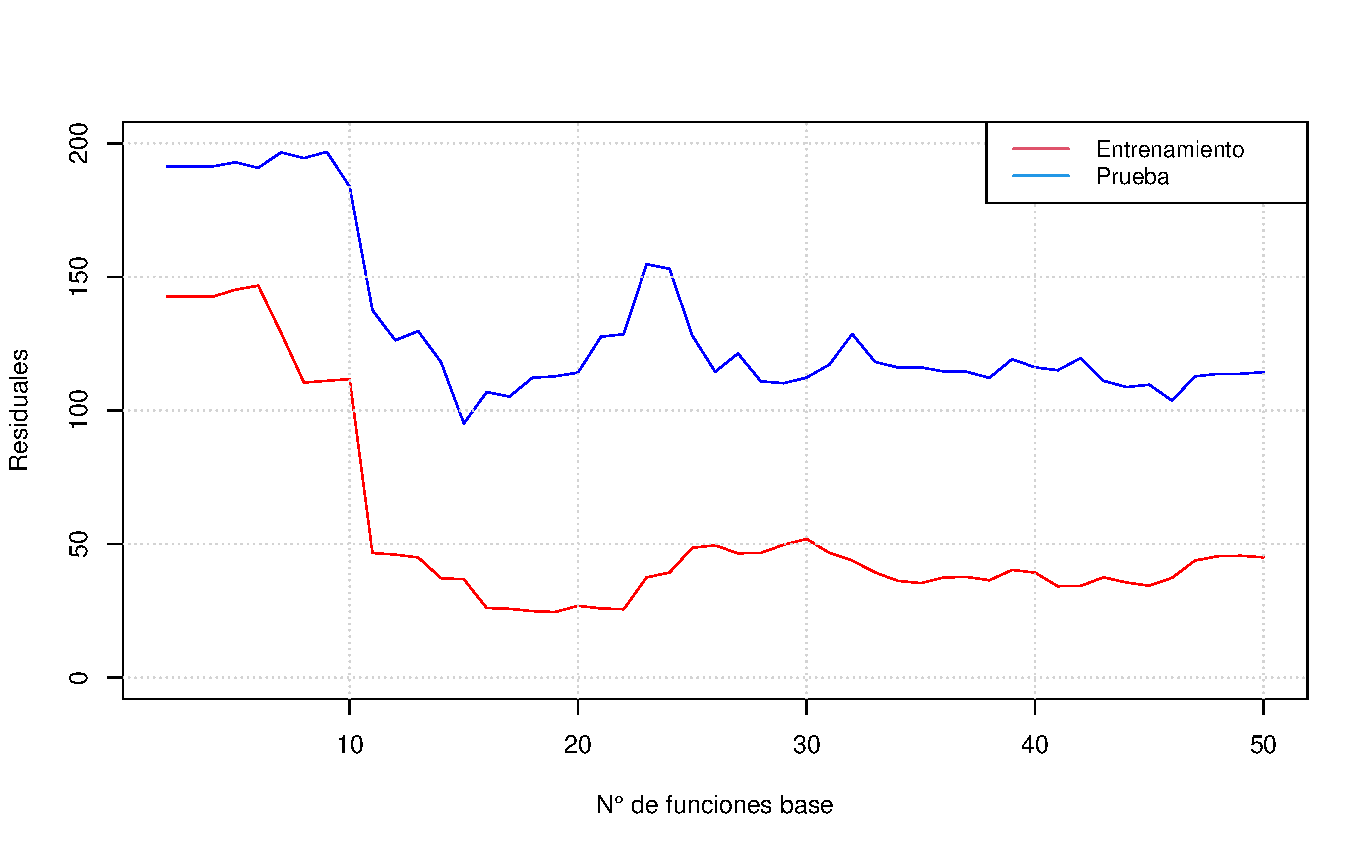
\includegraphics[width=0.67\textwidth]{graficos/intensity_population_residuals.pdf}
	\caption{Residuales en la población} \label{intensity_population_residuals}
\end{figure}

\begin{figure}[h]
	\centering
	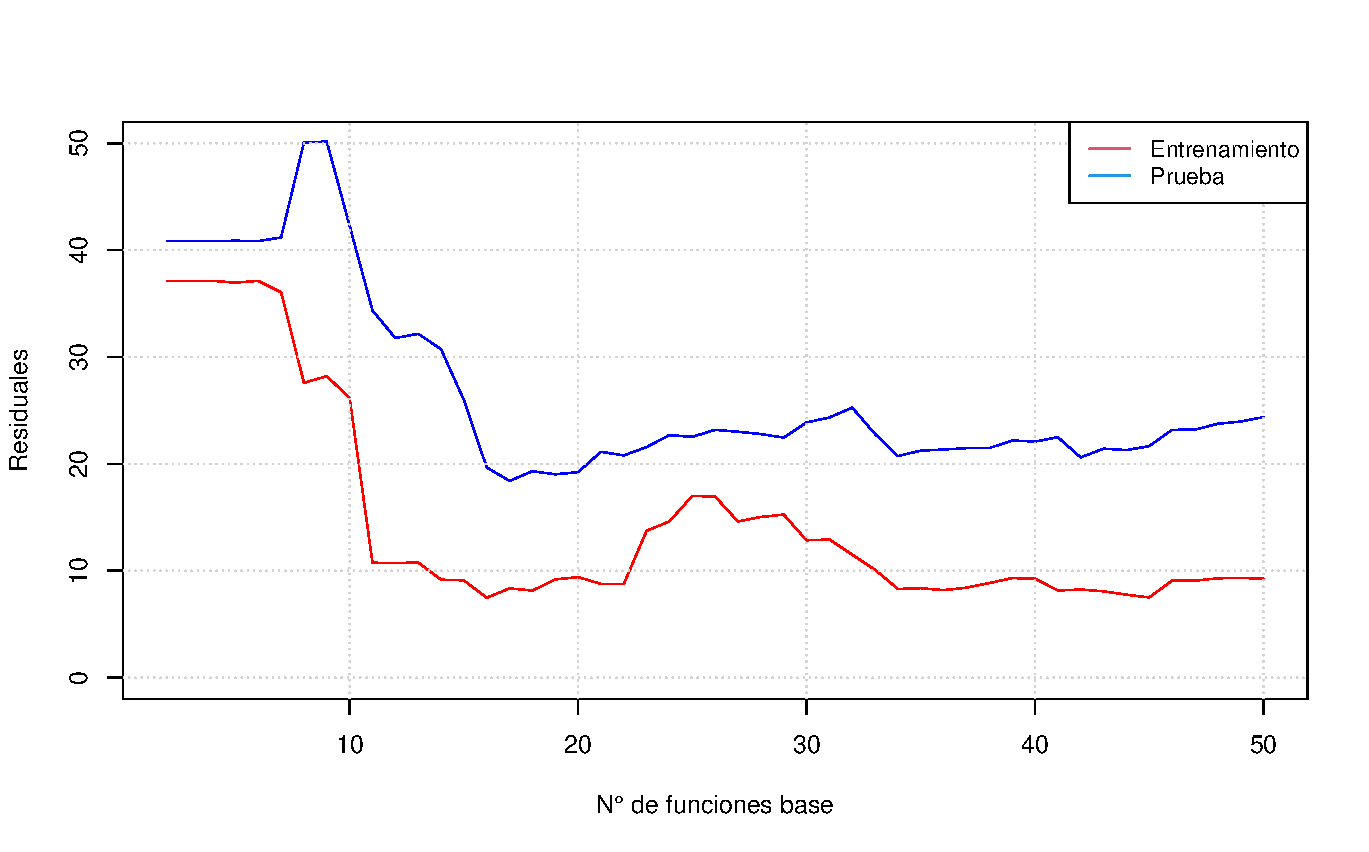
\includegraphics[width=0.67\textwidth]{graficos/intensity_sample_residuals.pdf}
	\caption{Residuales en la muestra} \label{intensity_sample_residuals}
\end{figure}

\newpage


\subsection{Riesgo}
Comparando las métricas de ajuste del grupo de entrenamiento y del grupo de prueba de cada modelo ajustado (Tabla~\ref{model_metricas}), se encontró una mejora en los modelos al introduccir el factor de corrección w, salvo aquel modelo que solo consideró el efecto espacial de las observaciones (Modelo espacial). Este mismo comportamiento se observó cuando a las covariables comprendidas como factores de riesgo (edad, sexo, tener al menos 3 perros) se les añadió la variable del efecto espacial. En base a estos resultados, se seleccionó al \textit{Modelo completo (w)}, compuesto por los factores de riesgo, el efecto espacial y el factor de correción w, como el modelo más adecuado para la inferencia y estimación del valor de la prevalencia corregida.

% Please add the following required packages to your document preamble:
% \usepackage{booktabs}
% \usepackage{multirow}
\begin{center}
	\begin{table}[h]
		\centering
		\caption{Métricas de ajuste para los modelos}
		\label{model_metricas}
		\begin{tabular}{@{}lcccccc@{}}
			\toprule
			\multicolumn{1}{c}{\multirow{2}{*}{Modelo}} & \multicolumn{3}{c}{Entrenamiento}                          & \multicolumn{3}{c}{Prueba}            \\ \cmidrule(l){2-7} 
			\multicolumn{1}{c}{}                        & Esp. & Sens. & \multicolumn{1}{c|}{AUC}    & Esp. & Sens. & AUC    \\ \midrule
			\multicolumn{1}{l|}{Modelo espacial}            & 1             & 0       & \multicolumn{1}{c|}{0.5381} & -       & -            & 0.6766 \\
			\multicolumn{1}{l|}{Modelo espacial (w)}            & 0.96             & 0.125       & \multicolumn{1}{c|}{0.5864} & -       & -            & 0.5453 \\
			\multicolumn{1}{l|}{Modelo edad}            & 1             & 0.0833       & \multicolumn{1}{c|}{0.5578} & 0.03125       & 1            & 0.5672 \\
			\multicolumn{1}{l|}{Modelo edad (w)}        & 0.9333        & 0.2917       & \multicolumn{1}{c|}{0.6122} & 0.59375       & 0.6          & 0.6453 \\
			\multicolumn{1}{l|}{Modelo sexo}            & 1             & 0            & \multicolumn{1}{c|}{0.5358} & 1             & 0            & 0.5469 \\
			\multicolumn{1}{l|}{Modelo sexo (w)}        & 1             & 0            & \multicolumn{1}{c|}{0.4642} & 1             & 0            & 0.5469 \\
			\multicolumn{1}{l|}{Modelo perros}          & 0.9333        & 0.3333       & \multicolumn{1}{c|}{0.6333} & 0.9688        & 0            & 0.149  \\
			\multicolumn{1}{l|}{Modelo perros (w)}      & 0.9333        & 0.3333       & \multicolumn{1}{c|}{0.6333} & 0.9688        & 0            & 0.149  \\
			\multicolumn{1}{l|}{Modelo sexo edad}       & 1             & 0.0833       & \multicolumn{1}{c|}{0.6369} & 0.03125       & 1            & 0.5406 \\
			\multicolumn{1}{l|}{Modelo sexo edad (w)}   & 0.9467        & 0.4583       & \multicolumn{1}{c|}{0.8708} & 0.5625        & 0.8          & 0.7562 \\
			\multicolumn{1}{l|}{Modelo s. e. p.}        & 0.96          & 0.375        & \multicolumn{1}{c|}{0.74}   & 0.0938        & 0.9          & 0.5141 \\
			\multicolumn{1}{l|}{Modeso s. e. p. (w)}    & 0.9467        & 0.4583       & \multicolumn{1}{c|}{0.7144} & 0.625         & 0.5          & 0.5328 \\
			\multicolumn{1}{l|}{Modelo completo}        & 0.96          & 0.333        & \multicolumn{1}{c|}{0.7403} & 0.53125       & 0.5          & 0.6    \\
			\multicolumn{1}{l|}{Modelo completo (w)}    & 0.9733        & 0.375        & \multicolumn{1}{c|}{0.7503} & 0.5625        & 0.8          & 0.7438 \\ \bottomrule
		\end{tabular}
	\end{table}
	
\end{center}

\newpage

\section{Infererencia}

El modelo final, \textit{modelo completo (w)}, fue utilizado para inferir la presencia de la enfermedad en los datos no muestreados. Con esto se pudo estimar una prevalencia corregida del 0.22. Este valor, si bien se encontraba dentro del intervalo de confianza para el primer estudio, estaba por debajo de su valor puntual (0.241), comportamiento que se ha visto repetido en el segundo estudio (0.235). Esto indicó la presencia de una sobrestimación en la prevalencia del primer estudio.


\begin{figure}[h]
	\centering
	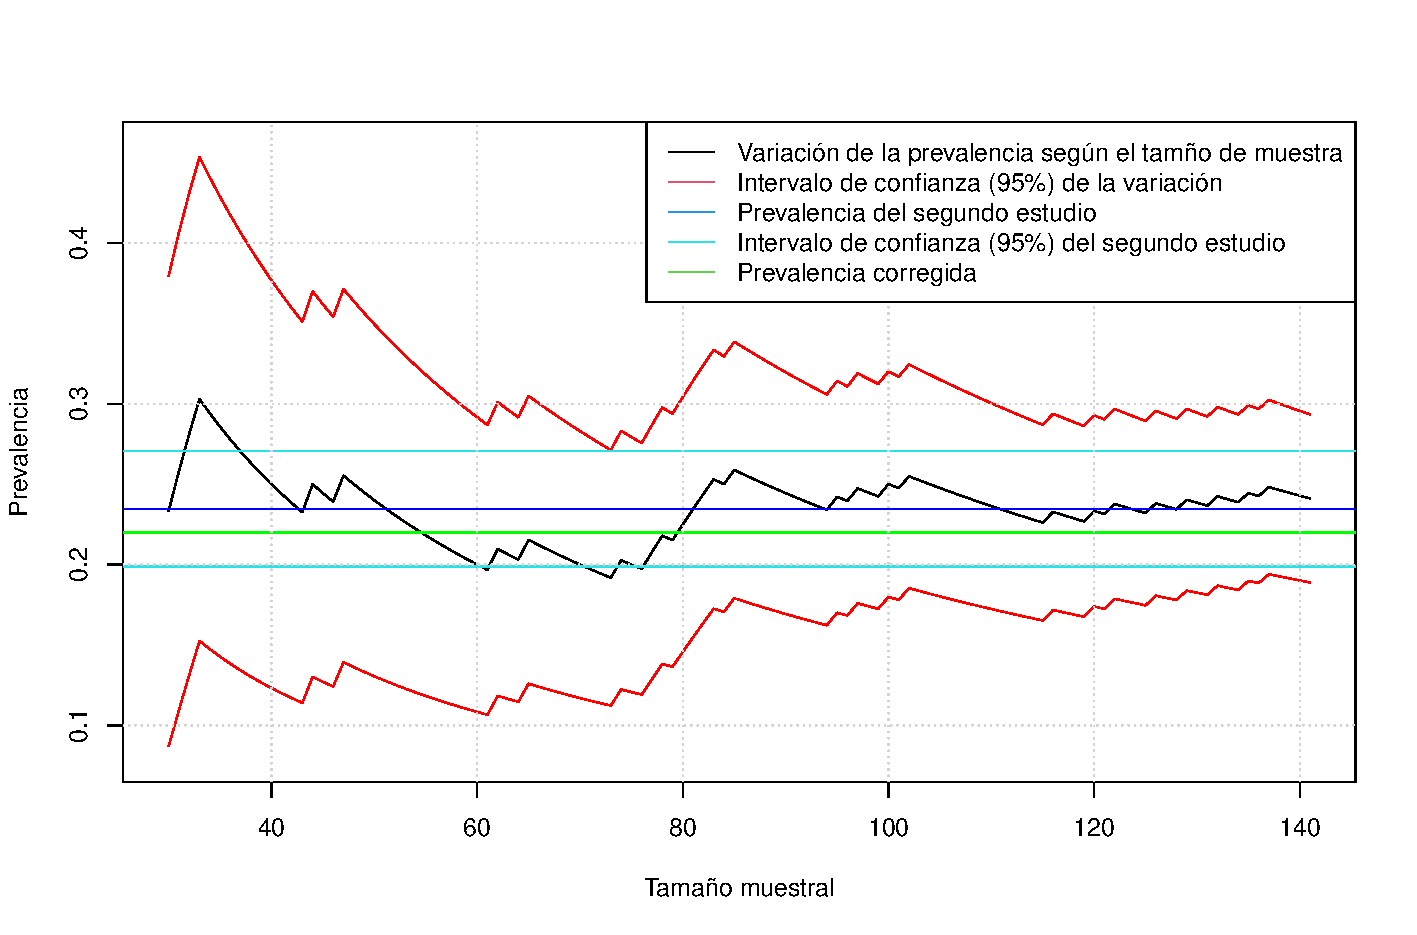
\includegraphics[width=1\textwidth]{graficos/prevalence_samplesize_fixed.pdf}
	\caption{Prevalencia de Hidatidosis Humana en Corpacancha, añadiendo la prevalencia corregida.}
	\label{prevalence_samplesize_fixed}
\end{figure}

\newpage
Esto permitió estimar un factor de corrección para la intesidad de $\rho$ = 1.126 (Véase~\ref{rho}). Empleando esto en~\ref{intesidad_rho}, se observó el cambio en el riesgo corregido de tener la enfermedad a nivel espacial en la población (Figura \ref{risk_to_disease_fixed}).
\begin{equation*}
	\hat{p}(x,y) = \cfrac{\hat{\lambda}_1(x,y)}{\hat{\lambda}_1(x,y)+ \rho \hat{\lambda}_0(x,y)} = \cfrac{\hat{\lambda}_1(x,y)}{\hat{\lambda}_1(x,y)+ 1.126* \hat{\lambda}_0(x,y)}
\end{equation*}

\begin{figure}[h]
	\centering
	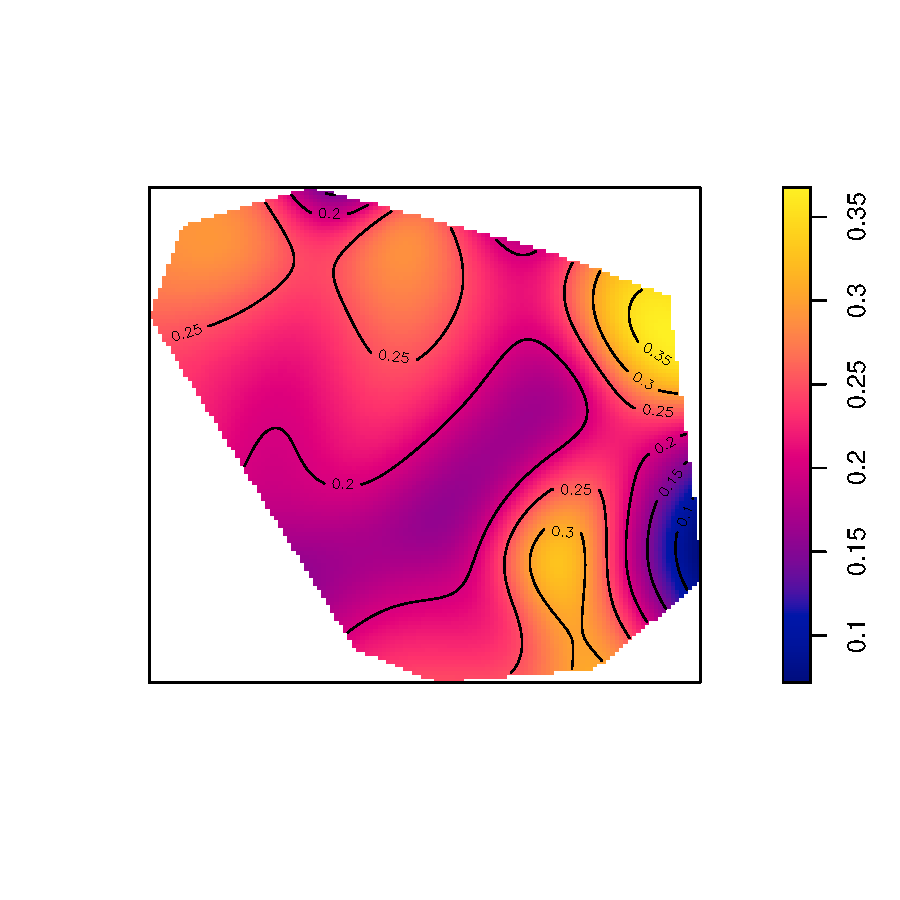
\includegraphics[width=0.9\textwidth]{graficos/risk_to_disease_fixed.pdf}
	\caption{Riesgo corregido de tener la enfermedad} \label{risk_to_disease_fixed}
\end{figure}




\newpage


\section{Implementación}
Con el fin de analizar la utilidad del método propuesto pero en otros contextos, se aplicó en el centro poblado de Canchayllo y se tuvo como resultado una prevalencia del $0.150$ ( $\pm 0.049$ IC$_{95\%}$  ).

\subsection*{Ajuste de intensidad}
Se ajustaron las intensidades correspondientes para la población y la muestra. El cociente de estas intensidades se puede ver en la Figura \ref{canchayllo_risk_to_sampling}, tal como en la sección \ref{seccion_intensidad}. La no homoegeniedad observada en esta figura se confirmó tras hacer la evaluación en base al algoritmo \ref{validaHipo}, debido a que en más de una observación, el cociente entre las dos intensidades no se ha encontrado en el intervalo de confianza correspondiente de acuerdo al algoritmo.


\begin{figure}[h]
	\centering
	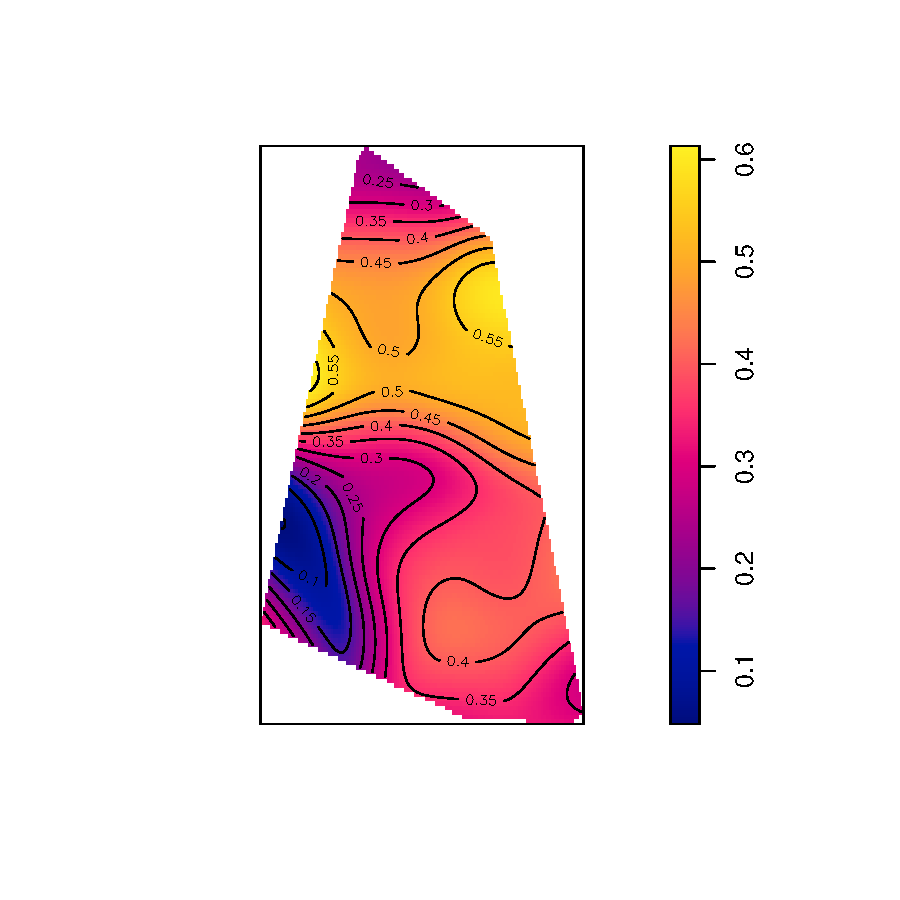
\includegraphics[width=0.7\textwidth]{graficos/canchayllo_risk_to_sampling.pdf}
	\caption{Riesgo de participar en la muestra en Canchayllo}
	\label{canchayllo_risk_to_sampling}
\end{figure}

\newpage

\begin{figure}[h]
	\centering
	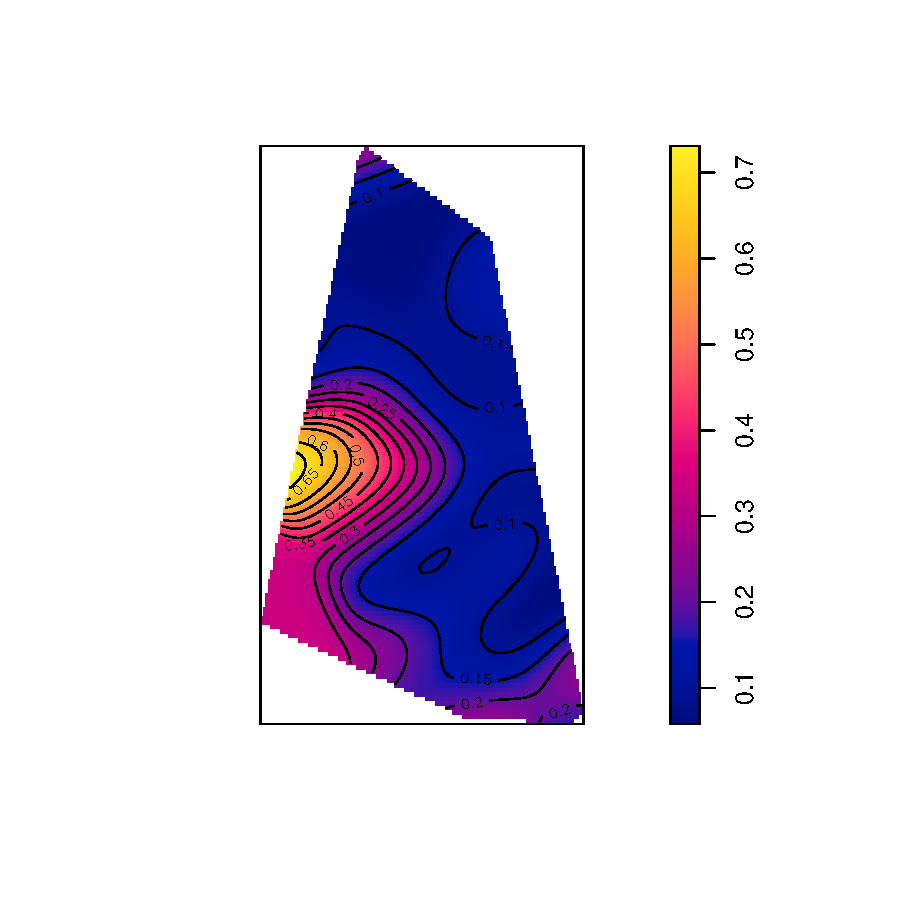
\includegraphics[width=0.7\textwidth]{graficos/canchayllo_risk_to_disease.pdf}
	\caption{Riesgo de la enfermedad en la muestra en Canchayllo}
	\label{canchayllo_risk_to_disease}
\end{figure}

\newpage

\subsection*{Ajuste del modelo}
Se seleccionó un modelo GAM usando los pesos obtenidos según la metodología propuesta. Se tomó como covariable a la tenencia de perros (Tener o no tener más de 3 perros). Este modelo tuvo un AUC de 0.664 y 0.763 para los datos de entrenamiento y prueba, respectivamente

\subsection*{Inferencia}

Tras haber hecho el ajuste correspondiente, se obtuvo una prevalencia corregida, la cual ascendió a 0.245. Asimismo, el riesgo espacial fue corregido, lo cual muestra una observable diferencia con el el riesgo antes de realiza la corrección. Además, se puede observar la zona en la que el riesgo se concentra.

\begin{figure}[h]
	\centering
	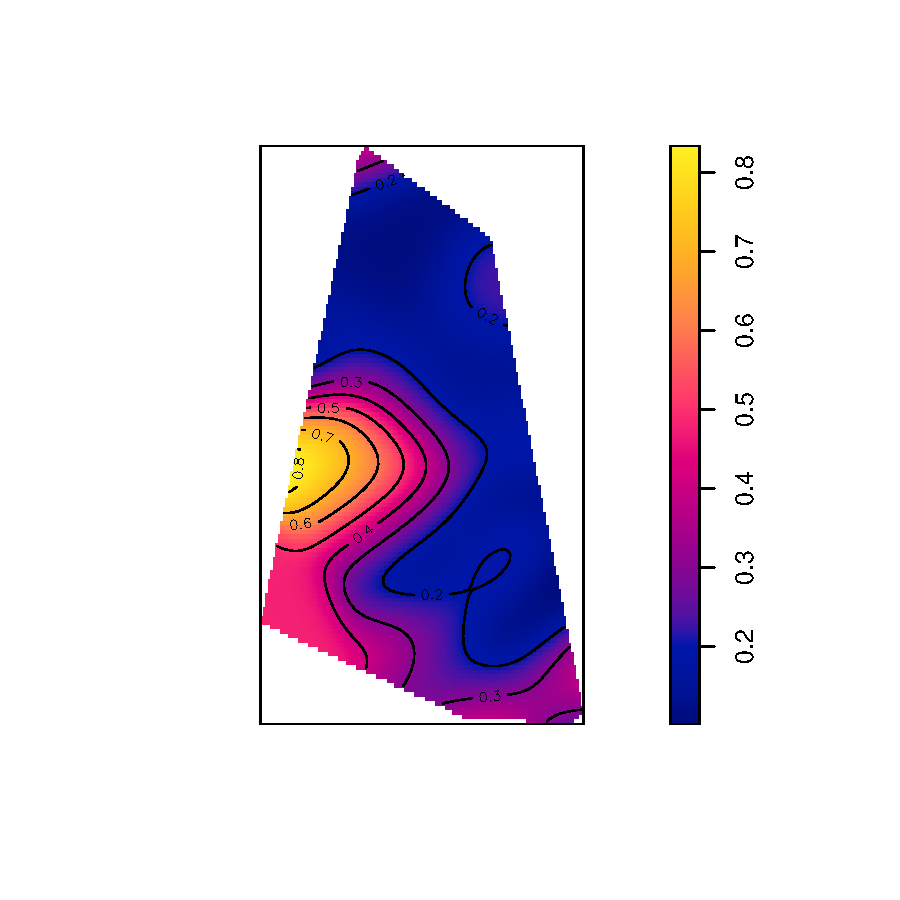
\includegraphics[width=0.7\textwidth]{graficos/canchayllo_risk_to_disease_fixed.pdf}
	\caption{Riesgo de la enfermedad en la muestra en Canchayllo}
	\label{canchayllo_risk_to_disease_fixed}
\end{figure}

%----------------------------------------------------------------------------------------
%	CONCLUSIONES Y RECOMENDACIONES
%----------------------------------------------------------------------------------------
\chapter{CONCLUSIONES Y RECOMENDACIONES}

\section{Conclusiones}

%\subsection{Respecto a los datos de la enfermedad}

Durante el análisis de las simulaciones se encontraron diferencias observables entre la distribución de la prevalencia estimada y la corregida. No obstante, y tal como se hizo mención en la sección de resultados, en un porcentaje notorio (más del 15\% en más de un escenario) el método propuesto para corregir la prevalencia obtuvo un resultado más cercano al real. En ese sentido, y considerando que estas simulaciones solo consideraron la componente espacial en la variabilidad de los datos y no otras covariables que permitan explicar su comportamiento, se concluyó de esta forma en que por el momento no existía la suficiente evidencia estadística que permita rechazar la hipótesis de que el método propuesto por lo general estima de una mejor forma la prevalencia que el método tradicional. \\
Por otro lado, de acuerdo a los resultados obtenidos en la prueba de Monte Carlo para la muestra correspondiente a la primera intervención en Corpacancha (la muestra no proviene de un muestreo totalmente aleatorio a nivel especial), se conocía que a causa de la no homogeneidad del riesgo espacial a ser seleccionados en la muestra era necesario utilizar un método que integre el factor espacial en el proceso de estimación de la prevalencia. Pese a los resultados obtenidos en el estudio del método planteado a través de las simulaciones, se aplicó con los datos reales. El método estudiado para corregir la prevalencia en el primer estudio generó resultados coherentes en relación a lo que el segundo estudio pudo obtener. En base a esto, se concluyó que la prevalencia del primer estudio (0.241) estuvo sobreestimada. El empleo del método presentado en esta investigación permitió poder estimar esta prevalencia de forma correcta al corregir el sesgo de selección. Al trabajar con la información recolectada en Canchayllo se determinó, en base a la prueba de Monte Carlo, un sesgo en la selección a nivel espacial, por lo que fue necesario emplear también el método propuesto para corregir con ello la prevalencia y el riesgo espacial a la enfermedad. Así, se concluyó que esta prevalencia se encontrada subestimada (0.245) debido al sesgo.\\
Durante la comparación de los modelos, se pudo observar que añadir el factor de ponderación \textit{w} por sí solo no obtenía una mejora en las métricas de ajuste. Por lo que fue necesario que este sea empleado en conjunto con los factores de riesgo. Esto evidenciaría la necesidad de no depender solo del análisis espacial al momento de buscar explicar la variabilidad de la información; sino también de la información sociodemográfica epidemiológica de los participantes del estudio.\\

%Por otro lado, durante el proceso de simulación, se obtuvieron resultados que debían de ser contrastados con lo optenido en el análisis de los datos reales para poder dar una conclusión correcta.


%razón por la cual en muchos casos, los modelos ajustados no tenían métricas de ajuste adecuadas.


%Faltaría añadir la discución de cómo estos resultado repercuten en la población


\newpage
\section{Recomendaciones}

Considerando lo planteando en la Sección \ref{enfteocon} y en base a las conclusiones presentadas, se recomienda que en estudios posteriores se plantee una prueba estadística que determine de forma objetiva el empleo de una metodología de corrección de sesgo espacial como la presentada. Para ello, la prueba debe estar vinculada al concepto de si el valor estimado de la prevalencia es insesgado y si el posible sesgo de selección se encuentra relacionado con el factor espacial u otra covariable. En este sentido, la prueba deberá evaluar si se rechaza o no la hipótesis nula de que la proporción de riesgo (PR) de la enfermedad entre el grupo seleccionado y el no seleccionado es 1.\\
%\begin{center}
%    \begin{itemize}
%        \item[] $\mathrm{H}_0: \;\mathrm{PR}\; =\; \cfrac{p(Y=1|X=1)}{p(Y=1|X=0)} \; = \; 1$
%        \item[] $\mathrm{H}_1: \;\mathrm{PR}\; =\; \cfrac{p(Y=1|X=1)}{p(Y=1|X=0)} \; \neq \; 1$
%    \end{itemize}
%\end{center}
De igual forma, se recomienda continuar en el estudio del método en sí bajo otros enfoques. En ello se tendría que analizar su comportamiendo al añadir covariables como factores de riesgo en diversas condiciones y distribuciones de los datos que sean distintas a las presentadas. En ese sentido, se podrá determinar los criterios mediantes los cuales el método pueda ser generalizado en estudios completamente diferentes. Con ello también poder desarrollar una regla de decisión que permita considerar invalida la muestra, basándose en la magnitud del sesgo de selección presente en ella.\\
Finalmente, también se recomienda hacer un estudio de impacto del método propuesto para determinar su viabilidad y su capacidad de implementabilidad en estudios epidemiológicos. Por ello se consideraría estudiar la rentabilidad del método, así como la importancia de su uso en el control, prevención y erradicación de enfermedades.

%\newpage

%\subsection{Implementación}




%----------------------------------------------------------------------------------------
%	REFERENCIA BIBLIOGRÁFICA
%----------------------------------------------------------------------------------------
\renewcommand*{\bibname}{REFERENCIA BIBLIOGRÁFICA}
\bibliography{references.bib}
\bibliographystyle{apacite}
%\bibliographystyle{acm} % estilo de la bibliografia
%\bibliography{bibliografia} % nombre del archivo .bib
%\addcontentsline{toc}{chapter}{REFERENCIA BIBLIOGRÁFICA}
\newpage


%----------------------------------------------------------------------------------------
%	ANEXOS
%----------------------------------------------------------------------------------------
\appendix
\clearpage
\addappheadtotoc
\appendixpage
\chapter{Aspectos legales}

\begin{figure}[h]
\centering
    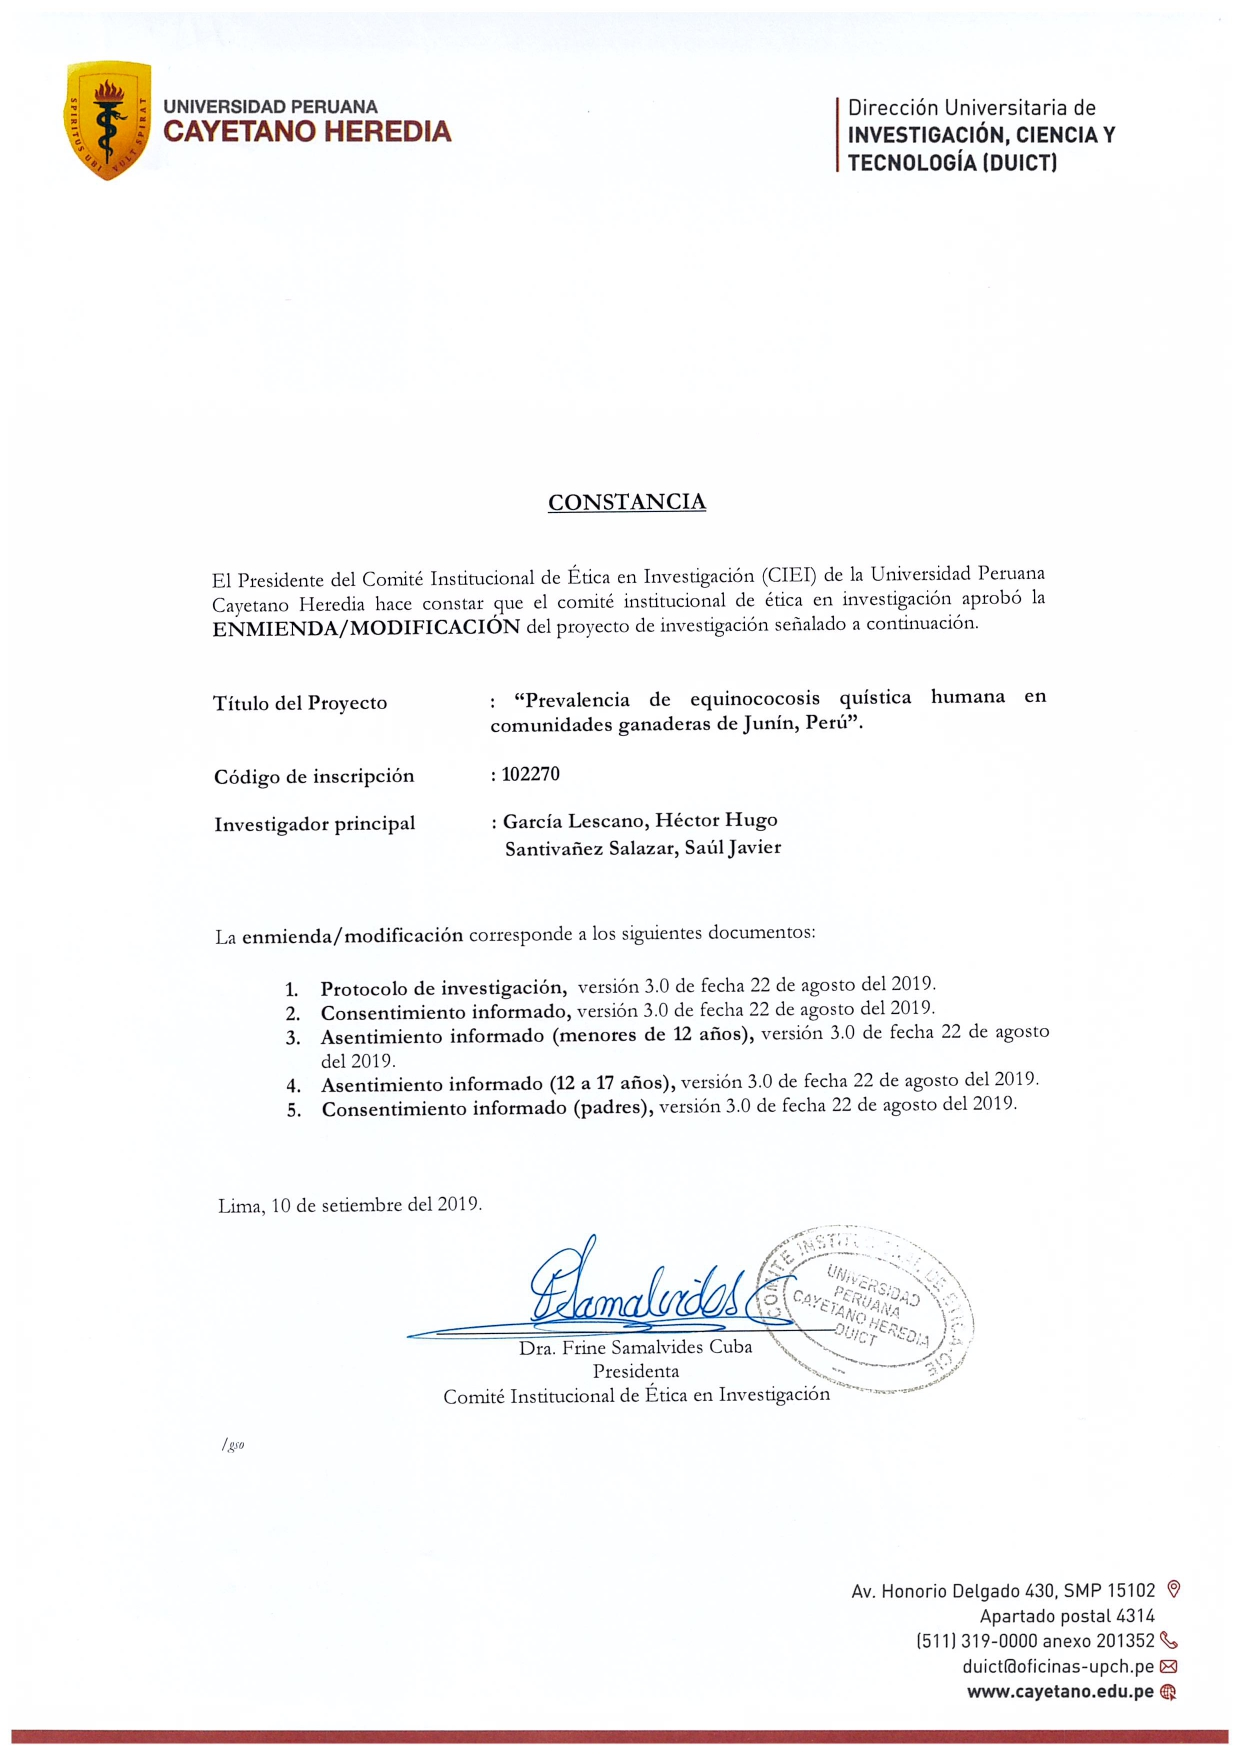
\includegraphics[width=0.5\textwidth]{imagenes/EM_AprobacionEtica.jpg}
    \caption{Carta de Aprobación Ética del Estudio Madre}
    \label{EM_apet}
\end{figure}

%\chapter{Diccionario de variables}\label{DicVar}

%Las variables que conformaron esta base de datos fueron:
%\begin{itemize}[noitemsep,nolistsep]
%    \item paciente: código autogenerado creado para mantener el anonimato del individuo
%    \item sexpac: Sexo del individuo
%    \item edapac: edad del individuo
%    \item ncasa: número de casa
%    \item virit\_wb: Tiene resultado de WB (Wester Blot) en el estudio VIRSEL
%    \item virit\_orden: Orden de participación en el estudio VIRSEL
%    \item virit\_resultado\_wb: Resultado del WB en el estudio VIRSEL
%    \item hycom\_particip: Participación en el estudio HYCOM
%    \item hycom\_orden: Orden de participación en el estudio HYCOM
%    \item hycom\_hid: Diagnostico de Hidatidos en el estudio HYCOM
%    \item hid\_corp: Diagnostico de Hidatidos en Corpacancha
%    \item rando\_edad: Rango de edad
%    \item longitud: Longitud (coordenada) de la casa
%    \item latitud: Latitud (coordenada) de la casa
%    \item distancia\_EsSalud: Distancia de la casa al centro de EsSalud
%\end{itemize}



\chapter{Códigos empleados para el desarrollo de la tesis}\label{CodR}


\begin{figure}[h]
	\centering
	
\includegraphics[width=0.5\textwidth]{imagenes/qr_codigo.png}
	\caption{QR enlazado al repositorio en GITHUB que contiene los códigos trabajados}
\end{figure}


\end{document} 


%http://www.mat.uda.cl/hsalinas/cursos/2008/latex/apuntes12.pdf
%http://metodos.fam.cie.uva.es/~latex/apuntes/apuntes3.pdf
%http://metodos.fam.cie.uva.es/~latex/apuntes/apuntes16.pdf
